\documentclass[svgnames, table, 10pt, aspectratio=169]{beamer} % aspectratio=1610, 149, 54, 43 et 32.]{beamer}
\usepackage{ae,lmodern}
\usepackage[english]{babel}  % package pour langue française
\usepackage[utf8]{inputenc} % compilation des mots accentués
\usepackage[T1]{fontenc}      % césure correcte des mots accentués 
\usepackage{eso-pic,rotating,graphicx} % insertion d'images et manipulation de la position
\usepackage{xcolor}
\usepackage[font=small]{caption}
\usepackage{subcaption} % utilisation d'une légende intermédiaire dans le cas d'une image multiple
\usepackage{url} % utilisation des liens url (utilisation dans le cas de la bibliographie par exemple
\usepackage{tcolorbox,listings} % coloration du texte et possibilité d'inclure blocs de codes
\usepackage{geometry} % customisation des layouts de page (marges, bordures, espacements)
\usepackage{amssymb} % caractères mathématiques
\usepackage{multirow, makecell} % tableau sur plusieurs colonnes fusionnées
\usepackage{bibentry}
\usepackage[backend=biber,style=numeric-comp, sorting=none, natbib=true]{biblatex} % exemples styles : https://fr.overleaf.com/learn/latex/Biblatex_bibliography_styles (mla pas mal)
\usepackage{comment} % utilisation des commentaires de blocs
\setcounter{tocdepth}{2} % profondeur du sommaire (2 = sections, sous sections)
\setcounter{secnumdepth}{1} % profondeur de la numérotation (1 : sections)
\usepackage{ragged2e} % justification du texte dans les itemizes
\usepackage{tikz} % création de schémas directement dans les slides
\usepackage{csquotes} % pour enlever un warning avec biblatex
\usepackage{fontawesome} %emoji
\usepackage{marvosym}
\usepackage[normalem]{ulem}
\usepackage{booktabs}
\usepackage{nth}
\usepackage{siunitx}

% William PENSEC, étudiant en Doctorat à Lorient 2021/2024

%-------- Lab-STICC Backgound -------------------
% \usebackgroundtemplate{%
% 	\tikz[overlay,remember picture] \node[opacity=0.02, at=(current page.center)] {
% 		
\includegraphics[width=4.5in]{images/logo/labsticc.png}};
% }


\usetheme[secheader]{Madrid}
\beamertemplatenavigationsymbolsempty
\setbeamertemplate{frametitle continuation}{}
\setbeamertemplate{caption}[numbered]
\setbeamertemplate{headline}


\definecolor{bleuLabSTICC}{RGB}{0,49,99}
\colorlet{beamer@blendedblue}{bleuLabSTICC}

\newcommand{\manualshortsubtitle}{PhD Defense - Lorient}

\makeatletter
\setbeamercolor{footlinecolor}{fg=bleuLabSTICC, bg=white}
\setbeamertemplate{footline}
{
  \leavevmode%
  \hbox{%
  \begin{beamercolorbox}[wd=.55\paperwidth,ht=2.75ex,dp=1ex,left]{footlinecolor}%
    \usebeamerfont{author in head/foot}\insertshortauthor (\insertshortinstitute)
  \end{beamercolorbox}
  \begin{beamercolorbox}[wd=.45\paperwidth,ht=2.75ex,dp=1ex,right]{footlinecolor}%
    \usebeamercolor{date in head/foot}\manualshortsubtitle~--~
    \usebeamerfont{date in head/foot}\insertdate{}\hspace*{2em}
    \insertframenumber{} / \inserttotalframenumber\hspace*{2ex} 
  \end{beamercolorbox}}%
  \vskip0pt%
}
\makeatother

\makeatletter
\setbeamercolor{frametitlecolor}{fg=bleuLabSTICC!75, bg=bleuLabSTICC!10}
\setbeamertemplate{frametitle}{%
  \nointerlineskip
  \begin{beamercolorbox}[sep=.3ex,wd=\paperwidth,leftskip=.5cm,rightskip=0cm]{frametitlecolor}%
    \usebeamerfont{frametitle}\insertframetitle\\[1pt]
  \end{beamercolorbox}
  \ifx\insertframesubtitle\@empty%
  \else
  \nointerlineskip%
  \begin{beamercolorbox}[sep=.3ex,wd=\paperwidth,leftskip=.5cm,rightskip=0cm]{frametitlecolor}%
  \usebeamerfont{framesubtitle}\usebeamercolor[fg]{framesubtitle}\insertframesubtitle%
  \end{beamercolorbox}
  \fi
}
\makeatother

\makeatletter
\setbeamertemplate{title page}{%
    \vfill
    \begingroup
    \centering
    \begin{beamercolorbox}[sep=8pt,center,rounded=true,shadow=false]{title}
        \usebeamerfont{title}\inserttitle\par%
        \ifx\insertsubtitle\@empty%
        \else%
            \vskip0.25em%
            {\usebeamerfont{subtitle}\usebeamercolor[fg]{subtitle}\insertsubtitle\par}%
        \fi%     
    \end{beamercolorbox}%
    \vskip1em\par
    \begin{beamercolorbox}[sep=8pt,center]{author}
        \usebeamerfont{author}\insertauthor
    \end{beamercolorbox}
    \vspace{-.25cm}% NEW
    \begin{beamercolorbox}[sep=8pt,center]{institute}
        \usebeamerfont{institute}\footnotesize\insertinstitute
    \end{beamercolorbox}
    \vspace{-.5cm}% NEW
    \begin{beamercolorbox}[sep=8pt,center]{date}
        \usebeamerfont{date}\footnotesize\insertdate
    \end{beamercolorbox}\vskip0.5em
    \begin{columns}
        \begin{column}{.4\linewidth}
            \centering \scriptsize
            \begin{tabular}{@{}rl@{}}
                % \toprule
                \multicolumn{2}{c}{\textbf{Composition of the Jury}} \\ \midrule
                % President of the jury:  & TBD                        \\
                Reviewers:              & Lejla BATINA               \\
                                        & Vincent BEROULLE           \\
                                        & Nele MENTENS               \\
                Examiners:              & Jean-Max DUTERTRE          \\
                                        & Francesco REGAZZONI        \\
                PhD supervisor:         & Guy GOGNIAT                \\
                PhD co-director:        & Vianney LAP\^OTRE          %\\ \bottomrule
            \end{tabular}
        \end{column}
        \begin{column}{.6\linewidth}
            {\usebeamercolor[fg]{titlegraphic}\inserttitlegraphic\par}
        \end{column}
    \end{columns}
    
    \endgroup
    \vfill
}
\makeatother

\makeatletter
\setbeamertemplate{back page}{%
    \vfill
    \begingroup
    \centering
    \begin{beamercolorbox}[sep=8pt,center,rounded=true,shadow=false]{title}
        \usebeamerfont{title}\inserttitle\par%   
    \end{beamercolorbox}%
    \vskip1em\par
    \begin{beamercolorbox}[sep=8pt,center]{author}
        \usebeamerfont{author}\insertauthor
    \end{beamercolorbox}
    \vspace{-.25cm}% NEW
    \begin{beamercolorbox}[sep=8pt,center]{institute}
        \usebeamerfont{institute}\footnotesize\insertinstitute
        \LARGE \textcolor{bleuLabSTICC!50}{Thank you for your attention.}
    \end{beamercolorbox}
    % \vspace{-.5cm}% NEW
    % \begin{beamercolorbox}[sep=8pt,center]{date}
    %     \usebeamerfont{date}\footnotesize\insertdate
    % \end{beamercolorbox}
    \vskip0.5em
    \begin{columns}
        \begin{column}{.4\linewidth}
            \centering \scriptsize
            \begin{tabular}{@{}rl@{}}
                % \toprule
                \multicolumn{2}{c}{\textbf{Composition of the Jury}} \\ \midrule
                % President of the jury:  & TBD                        \\
                Reviewers:              & Lejla BATINA               \\
                                        & Vincent BEROULLE           \\
                                        & Nele MENTENS               \\
                Examiners:              & Jean-Max DUTERTRE          \\
                                        & Francesco REGAZZONI        \\
                PhD supervisor:         & Guy GOGNIAT                \\
                PhD co-director:        & Vianney LAP\^OTRE          %\\ \bottomrule
            \end{tabular}
        \end{column}
        \begin{column}{.6\linewidth}
            {\usebeamercolor[fg]{titlegraphic}\inserttitlegraphic\par}
        \end{column}
    \end{columns}
    
    \endgroup
    \vfill
}
\makeatother

% Define backpage command
\newcommand{\backpage}{
    \usebeamertemplate{back page}
}

\hypersetup{
  % hidelinks,
  colorlinks=true,       % false: boxed links; true: colored links
  linkcolor=bleuLabSTICC,          % color of internal links (change box color with linkbordercolor)
  citecolor=red,        % color of links to bibliography
  filecolor=black,         % color of file links
  urlcolor=bleuLabSTICC,        % color of external links
  pdfauthor = {William PENSEC},			                        % Auteurs
  pdftitle = {Enhanced Processor Defence Against Physical and Software Threats by Securing DIFT Against Fault Injection Attacks},	% Titre du document
  pdfsubject = {PhD Dissertation Defense},		            % Sujet
  pdfkeywords = {Hardware security, DIFT, Fault Injection Attacks, Countermeasures, Error Correction Code, Error Detection Code, Embedded Processor},  % Mots-clefs
  pdfstartview={FitV}                                         % ajuste la page à la largueur de l'écran
}

\bibliography{bib/bibliographie.bib}
\renewcommand*{\bibfont}{\footnotesize}

% \AtBeginSection[] {
%   \begin{frame}[noframenumbering, plain]{Outline}
%     \vfill % Centres vertically
%     \tableofcontents[
%       currentsection,
%       currentsubsection,
%       hideothersubsections,
%       sectionstyle=show/shaded,
%       sections={\thesection}
%     ]
%     \vfill
%   \end{frame}
% }

\defbeamertemplate{section in toc}{sections numbered roman}{%
  \leavevmode%
  \MakeUppercase{\romannumeral\inserttocsectionnumber}.\ \inserttocsection\par
}
\defbeamertemplate{subsection in toc}{subsections numbered alone}{%
  \leavevmode%
  \hspace{1em}\inserttocsubsectionnumber.\ \inserttocsubsection\par
}

\setbeamertemplate{section in toc}[sections numbered roman]
\setbeamertemplate{subsection in toc}[subsections numbered alone]

\AtBeginSection[]{
  \begin{frame}{}
    \vfill
    % \centering
    % \begin{beamercolorbox}[sep=8pt,center,shadow=true,rounded=true]{title}
    %     \Huge\tableofcontents[sectionstyle=show/hide, hideallsubsections]
    % \end{beamercolorbox}
    \begin{center}
        \Huge \tableofcontents[sectionstyle=show/hide, hideallsubsections]
    \end{center}
    \vfill
  \end{frame}
}

\newcommand{\filigrane}[3]{\begin{tikzpicture}[remember picture,overlay]
	\node [rotate=#2,scale=#3,text opacity=0.75]
	at (current page.center) {\textcolor{red}{\textbf{#1}}};
	\end{tikzpicture}
}

% Define color
\definecolor[named]{LightGray}{RGB}{230,230,230}

\setbeamercovered{transparent}

\newcommand{\tableTwoLines}[2]{\begin{tabular}[c]{@{}c@{}}#1\\ #2\end{tabular}}
\newcommand{\tableCentered}[1]{\begin{tabular}[c]{@{}c@{}}#1\end{tabular}}
\captionsetup{font=footnotesize}
\definecolor{backcolour}{rgb}{0.98,0.98,0.98}
\definecolor[named]{LightGray}{RGB}{230,230,230}

\lstset{
  aboveskip=0.25cm,
  belowskip=0mm,
  basicstyle=\tiny,
  backgroundcolor=\color{backcolour},
  breakatwhitespace=false,
  breaklines=true,
  captionpos=t,
  commentstyle=\color{gray},
  deletekeywords={...},
  escapeinside={\%*}{*)},
  extendedchars=true,
  framexleftmargin=1pt,
  framextopmargin=0pt,
  framexbottommargin=0pt,
  frame=tb,
  keepspaces=true,
  keywordstyle=\color{red},
  language=C,
  literate=
  {²}{{\textsuperscript{2}}}1
  {⁴}{{\textsuperscript{4}}}1
  {⁶}{{\textsuperscript{6}}}1
  {⁸}{{\textsuperscript{8}}}1
  {€}{{\euro{}}}1
  {é}{{\'e}}1
  {è}{{\`{e}}}1
  {ê}{{\^{e}}}1
  {ë}{{\"{e}}}1
  {É}{{\'{E}}}1
  {Ê}{{\^{E}}}1
  {û}{{\^{u}}}1
  {ù}{{\`{u}}}1
  {â}{{\^{a}}}1
  {à}{{\`{a}}}1
  {á}{{\'{a}}}1
  {ã}{{\~{a}}}1
  {Á}{{\'{A}}}1
  {Â}{{\^{A}}}1
  {Ã}{{\~{A}}}1
  {ç}{{\c{c}}}1
  {Ç}{{\c{C}}}1
  {õ}{{\~{o}}}1
  {ó}{{\'{o}}}1
  {ô}{{\^{o}}}1
  {Õ}{{\~{O}}}1
  {Ó}{{\'{O}}}1
  {Ô}{{\^{O}}}1
  {î}{{\^{i}}}1
  {Î}{{\^{I}}}1
  {í}{{\'{i}}}1
  {Í}{{\~{Í}}}1,
  morekeywords={},
  numbers=left,
  numbersep=10pt,
  numberstyle=\tiny\color{black},
  rulecolor=\color{black},
  showspaces=false,
  showstringspaces=false,
  showtabs=false,
  stepnumber=1,
  stringstyle=\color{gray},
  tabsize=4,
  title=\lstname
}

\lstdefinestyle{topPosition}{
  float=ht,
  floatplacement=ht
}

\colorlet{punct}{red!60!black}
% \definecolor{background}{HTML}{EEEEEE}
\definecolor{delim}{RGB}{0,0,255}
\colorlet{numb}{magenta!60!black}
\lstdefinelanguage{json}{
    basicstyle=\tiny,
    numbers=left,
    numberstyle=\tiny,
    stepnumber=1,
    numbersep=8pt,
    showstringspaces=false,
    breaklines=true,
    frame=lines,
    literate=
     *{0}{{{\color{numb}0}}}{1}
      {1}{{{\color{numb}1}}}{1}
      {2}{{{\color{numb}2}}}{1}
      {3}{{{\color{numb}3}}}{1}
      {4}{{{\color{numb}4}}}{1}
      {5}{{{\color{numb}5}}}{1}
      {6}{{{\color{numb}6}}}{1}
      {7}{{{\color{numb}7}}}{1}
      {8}{{{\color{numb}8}}}{1}
      {9}{{{\color{numb}9}}}{1}
      {:}{{{\color{punct}{:}}}}{1}
      {,}{{{\color{punct}{,}}}}{1}
      {\{}{{{\color{delim}{\{}}}}{1}
      {\}}{{{\color{delim}{\}}}}}{1}
      {[}{{{\color{delim}{[}}}}{1}
      {]}{{{\color{delim}{]}}}}{1},
}

\lstdefinelanguage[RISC-V]{Assembler}
{
  alsoletter={.}, % allow dots in keywords
  alsodigit={0x}, % hex numbers are numbers too!
  morekeywords=[1]{ % instructions
    lb, lh, lw, lbu, lhu,
    sb, sh, sw,
    sll, slli, srl, srli, sra, srai,
    add, addi, sub, lui, auipc,
    xor, xori, or, ori, and, andi,
    slt, slti, sltu, sltiu,
    beq, bne, blt, bge, bltu, bgeu,
    j, jr, jal, jalr, ret,
    scall, break, nop, 
    csrr
  },
  morekeywords=[2]{ % sections of our code and other directives
    .align, .ascii, .asciiz, .byte, .data, .double, .extern,
    .float, .globl, .half, .kdata, .ktext, .set, .space, .text, .word, mcycle
  },
  morekeywords=[3]{ % registers
    zero, ra, sp, gp, tp, s0, fp,
    t0, t1, t2, t3, t4, t5, t6,
    s1, s2, s3, s4, s5, s6, s7, s8, s9, s10, s11,
    a0, a1, a2, a3, a4, a5, a6, a7,
    ft0, ft1, ft2, ft3, ft4, ft5, ft6, ft7,
    fs0, fs1, fs2, fs3, fs4, fs5, fs6, fs7, fs8, fs9, fs10, fs11,
    fa0, fa1, fa2, fa3, fa4, fa5, fa6, fa7,
    x0, x1, x2, x3, x4, x5, x6, x7, x8, x9, 
    x10, x11, x12, x13, x14, x15, x16, x17, x18, x19,
    x20, x21, x22, x23, x24, x25, x26, x27, x28, x29,
    x30, x31
  },
  morecomment=[l]{;},   % mark ; as line comment start
  morecomment=[l]{\#},  % as well as # (even though it is unconventional)
  morestring=[b]",      % mark " as string start/end
  morestring=[b]'       % also mark ' as string start/end
}

% usage example:

% define some basic colors
\definecolor{mauve}{rgb}{0.58,0,0.82}

% \lstset{
%   basicstyle=\tiny\ttfamily,                    % very small code
%   breaklines=true,                              % break long lines
%   commentstyle=\itshape\color{green!50!black},  % comments are green
%   keywordstyle=[1]\color{blue!80!black},        % instructions are blue
%   keywordstyle=[2]\color{orange!80!black},      % sections/other directives are orange
%   keywordstyle=[3]\color{red!50!black},         % registers are red
%   stringstyle=\color{mauve},                    % strings are from the telekom
%   identifierstyle=\color{teal},                 % user declared addresses are teal
%   frame=l,                                      % black line on the left side of code
%   language=[RISC-V]Assembler,                   % all code is RISC-V
%   tabsize=4,                                    % indent tabs with 4 spaces
%   showstringspaces=false                        % do not replace spaces with weird underlines
% }
\title{Enhanced Processor Defence Against Physical and Software Threats by Securing DIFT Against Fault Injection Attacks}
\subtitle{PhD Dissertation Defense}
\author[
    William PENSEC
]{
    \textbf{William PENSEC}
}
\institute[Lab-STICC] % (optional)
{
    {\small Université Bretagne Sud, UMR 6285, Lab-STICC, Lorient, France} \\ \vspace{2mm}
}
\date{December 19, 2024}

% Multiple logos
\titlegraphic{
    
\includegraphics[height=1cm]{img/logo/ubs.png}
    \hspace{2cm}
    
\includegraphics[height=1cm]{img/logo/labsticc.pdf}
    \hspace{2cm}
    \includegraphics[height=1cm]{img/logo/cnrs.pdf}
}
% \setbeameroption{show notes on second screen = left}


\begin{document}
% ---------------------------------------------------------------- %
\begin{frame}[plain]
	\titlepage
\end{frame}
% ---------------------------------------------------------------- %
\section{Introduction}

%%%%%%%%%%%%%%%%%%%%%%%%%%%%%%%%%%%%%%%%%%%%%%%%%%%%%%%%%%%%%%%%%%%%%%%%%%%%
\begin{frame}{Context: IoT and Embedded Systems}
    
\end{frame}

%%%%%%%%%%%%%%%%%%%%%%%%%%%%%%%%%%%%%%%%%%%%%%%%%%%%%%%%%%%%%%%%%%%%%%%%%%%%
\begin{frame}{Motivations}
    
\end{frame}
%%%%%%%%%%%%%%%%%%%%%%%%%%%%%%%%%%%%%%%%%%%%%%%%%%%%%%%%%%%%%%%%%%%%%%%%%%%%
\begin{frame}{Objectives}
    
\end{frame}
%%%%%%%%%%%%%%%%%%%%%%%%%%%%%%%%%%%%%%%%%%%%%%%%%%%%%%%%%%%%%%%%%%%%%%%%%%%%
%
% ---------------------------------------------------------------- %
\begin{frame}{Outline}
	\begin{columns}
		\begin{column}{.15\linewidth}
			\hfill
		\end{column}
		\begin{column}{.8\linewidth}
			\Large\tableofcontents[hideallsubsections]
		\end{column}
		\begin{column}{.1\linewidth}
			\hfill
		\end{column}
	\end{columns}
\end{frame}
%
% ---------------------------------------------------------------- %
\section{D-RI5CY -- Vulnerability Assessment}

%%%%%%%%%%%%%%%%%%%%%%%%%%%%%%%%%%%%%%%%%%%%%%%%%%%%%%%%%%%%%%%%%%%%%%%%%%%%
\subsection{D-RI5CY - origins and architecture}
\begin{frame}{D-RI5CY - origins}
    \begin{itemize}
        \item Design~\cite{PDGLC-18-hpec} made by researchers at Columbia University (USA) with Politecnico di Torino (Italy)
        \item Based on the 32-bit RISC-V processor: RI5CY (Pulp Platform)
        \item Open source\footnote{\url{https://github.com/sld-columbia/riscv-dift}}
        \item 1-bit tag datapath
        \item Flexible security policy that can be modified at runtime
    \end{itemize}

    \centering
    \vfill
    
\includegraphics[height=1cm]{img/logo/riscv.png}
    \hspace{1cm}
    
\includegraphics[height=1cm]{img/logo/pulp_logo.pdf}
    \vfill
\end{frame}
%%%%%%%%%%%%%%%%%%%%%%%%%%%%%%%%%%%%%%%%%%%%%%%%%%%%%%%%%%%%%%%%%%%%%%%%%%%%
\begin{frame}{D-RI5CY - architecture}
    \begin{figure}
        \centering
        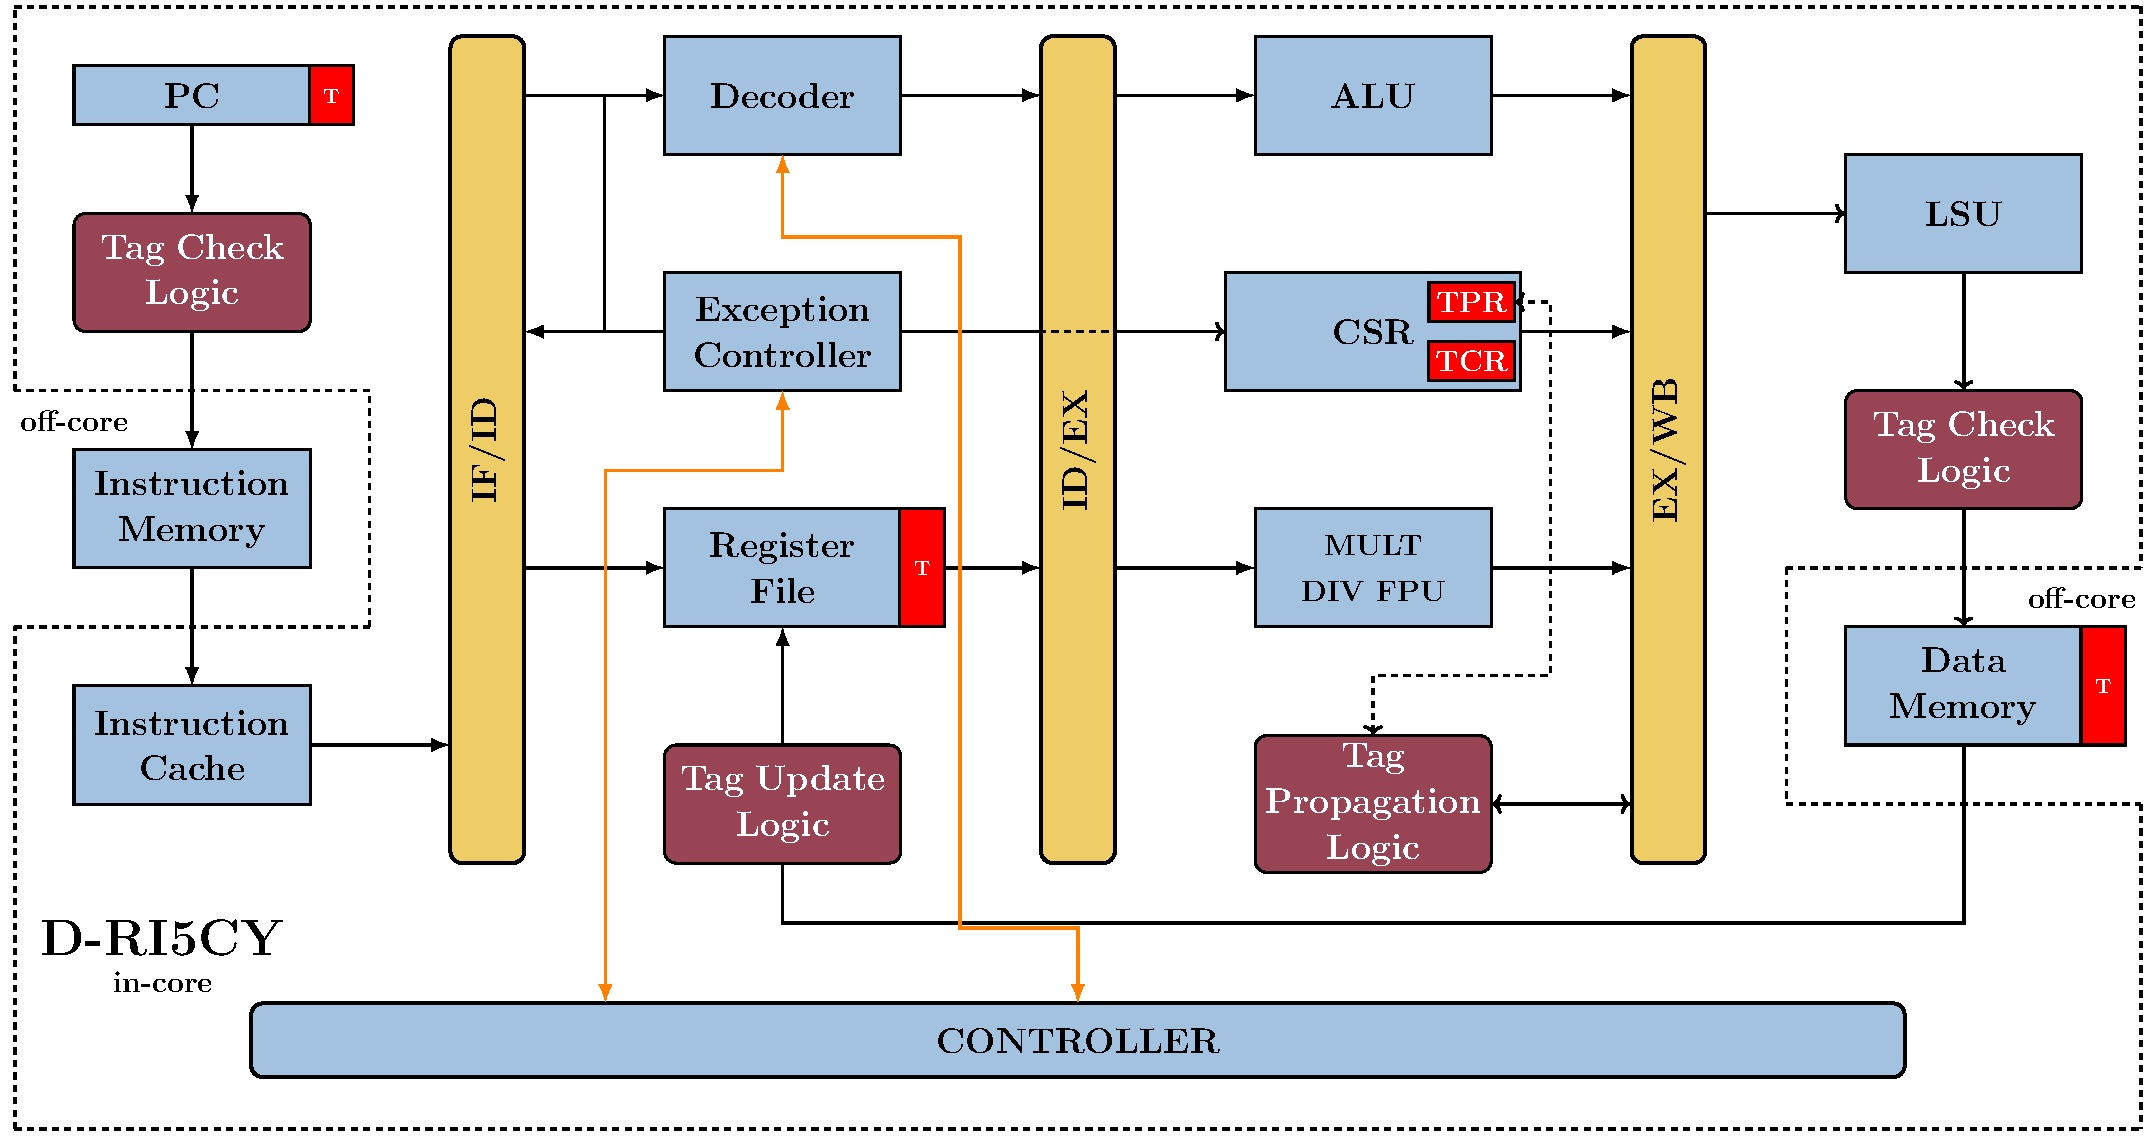
\includegraphics[width=.9\textwidth]{src/2_vuln_assessment/img/RI5CY.pdf}
        \caption{Architecture of the D-RI5CY.}
        \label{fig:riscy}
    \end{figure}
\end{frame}
%%%%%%%%%%%%%%%%%%%%%%%%%%%%%%%%%%%%%%%%%%%%%%%%%%%%%%%%%%%%%%%%%%%%%%%%%%%%
\subsection{Vulnerability assessment}
\begin{frame}{Vulnerability Assessment}
    \begin{block}{Threat model}
        We consider an attacker able to:
        \begin{itemize}
            \item perform a physical attack to defeat the DIFT mechanism and realise a software attack,
            \item inject faults in DIFT-related registers:
                  \begin{itemize}
                      \item bit set,
                      \item bit reset,
                      \item bit-flip.
                  \end{itemize}
        \end{itemize}
    \end{block}

    % \begin{block}{Methodology}
    %     \begin{itemize}
    %         \item Analysis of 2 attacks use cases: buffer overflow attack, format string attack
    %         \item Analysis of 1 use case to complete the DIFT surface: compare/compute
    %     \end{itemize}
    % \end{block}
\end{frame}
%%%%%%%%%%%%%%%%%%%%%%%%%%%%%%%%%%%%%%%%%%%%%%%%%%%%%%%%%%%%%%%%%%%%%%%%%%%%
\subsection{Use case : presentation}
\begin{frame}{Case 1: Buffer overflow}
    \begin{itemize}
        \item The attacker exploits a buffer overflow to access the return address register ($RA$).
    \end{itemize}

    \begin{figure}
        \centering
        \begin{subfigure}[l]{.45\textwidth}
            \centering
            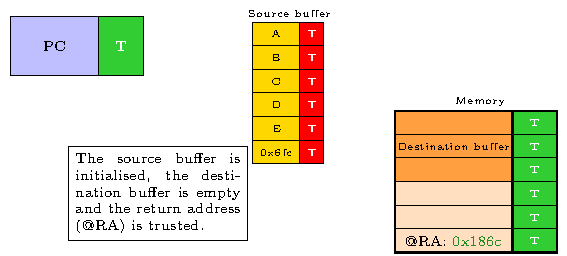
\includegraphics[width=.9\textwidth, page=1]{src/2_vuln_assessment/img/buffer_overflow/schemaPedagogique.pdf}
            \caption{Malicious buffer and $RA$ trusted}
            \label{fig:bo_1st_step}
        \end{subfigure}
        \begin{subfigure}[r]{.45\textwidth}
            \centering
            \includegraphics[width=.9\textwidth, page=5]{src/2_vuln_assessment/img/buffer_overflow/schemaPedagogique.pdf}
            \caption{Overflow and overwriting of $RA$ and its tag}
            \label{fig:bo_3rd_step}
        \end{subfigure}
    \end{figure}

    \begin{itemize}
        \item As the data in the source buffer is manipulated by the user, it is marked as \textcolor{red}{\textit{untrusted}}.
        \item Thanks to DIFT, the tags associated with the source buffer data overwrite the $RA$ register tag.
        \item When the function returns, the corrupted register $RA$ is loaded into $PC$ using a jalr instruction.
    \end{itemize}
\end{frame}

\begin{frame}
    \begin{figure}
        \centering
        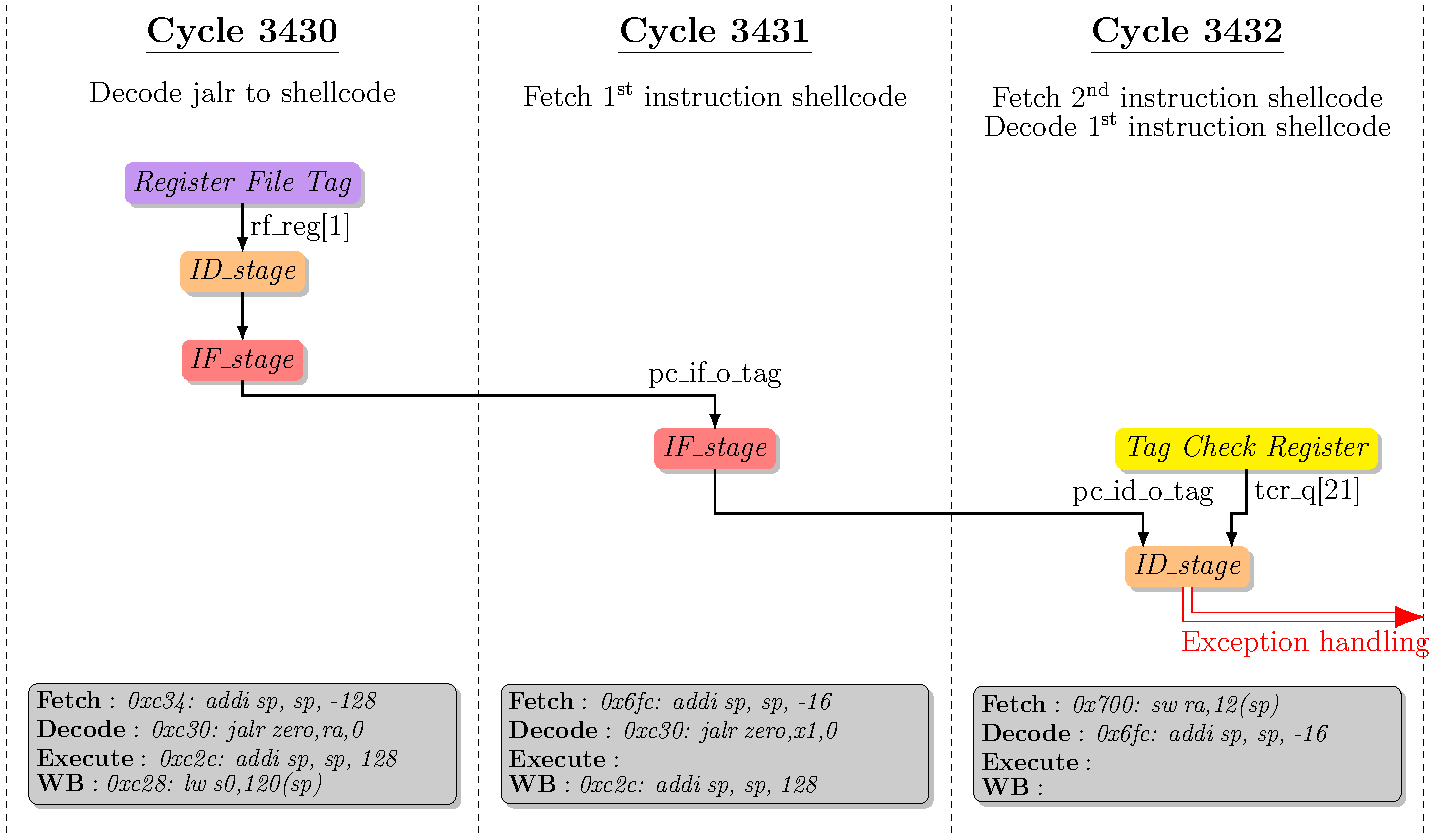
\includegraphics[width=.75\textwidth]{src/2_vuln_assessment/img/buffer_overflow/bufferOverflowAttack_short.pdf}
        \caption{Temporal analysis of the tags propagation in \textit{Buffer Overflow} attack}
        \label{fig:analyseTempoBufferOverflow}
    \end{figure}
\end{frame}

\begin{frame}
    \begin{figure}
        \centering
        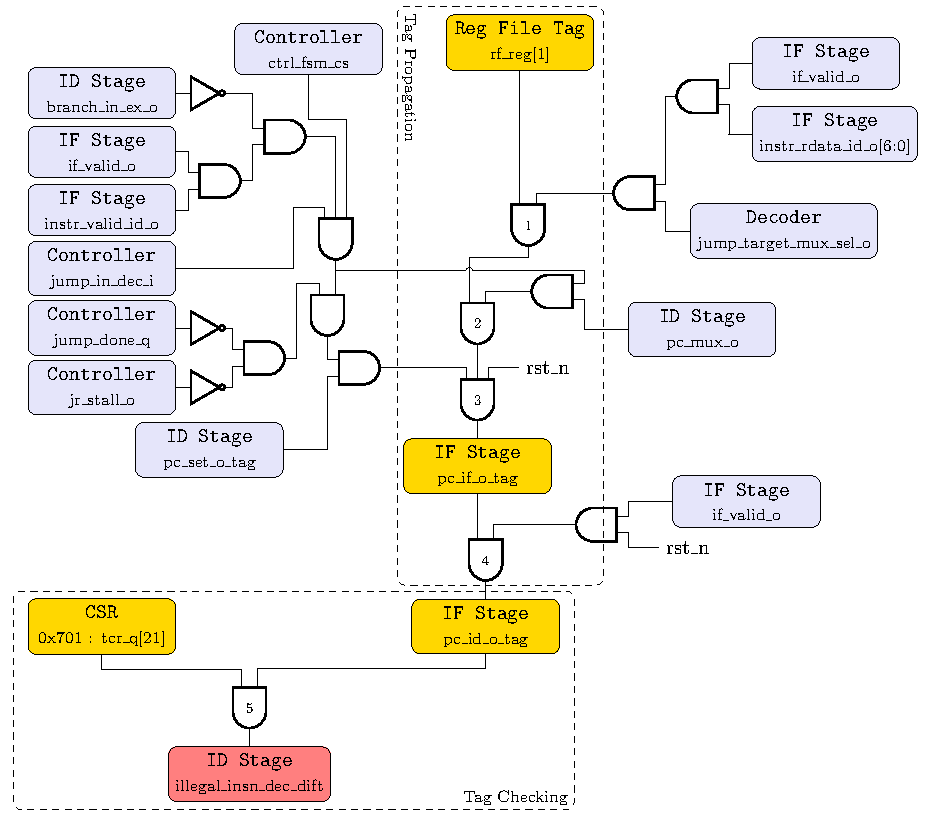
\includegraphics[height=.85\textheight]{src/2_vuln_assessment/img/buffer_overflow/arborescence_bufferOverflow.pdf}
        \caption{Logical analysis of the tags propagation in a \textit{Buffer Overflow} attack}
        \label{fig:analyseLogiqueBufferOverflow}
    \end{figure}
\end{frame}
%%%%%%%%%%%%%%%%%%%%%%%%%%%%%%%%%%%%%%%%%%%%%%%%%%%%%%%%%%%%%%%%%%%%%%%%%%%%%%%%%%%%%%%%%%%%%%%%%%%%%%%%%%%%
\begin{frame}[fragile]{Case 2: WU-FTPd}
    \begin{itemize}
        \justifying
        \item The vulnerability is the use of an unchecked user input as the format string parameter in functions that perform formatting, e.g. printf()
        \item An attacker can use the format tokens, to write into arbitrary locations of memory, e.g. the return address of the function.
    \end{itemize}

    % \vspace{1cm}
    % \hspace{2cm}
    \centering
    \begin{minipage}[c]{\textwidth}
        \begin{lstlisting}[language=C,label=code:printfNFormat]
void echo(){
    int a;
    register int i asm("x8");
    a = i;
    printf("%224u%n%35u%n%253u%n%n", 1, (int*) (a-4), 1, (int*) (a-3), 1, (int*) (a-2), (int*) (a-1));
}\end{lstlisting}
    \end{minipage}
\end{frame}

\begin{frame}
    \begin{figure}
        \centering
        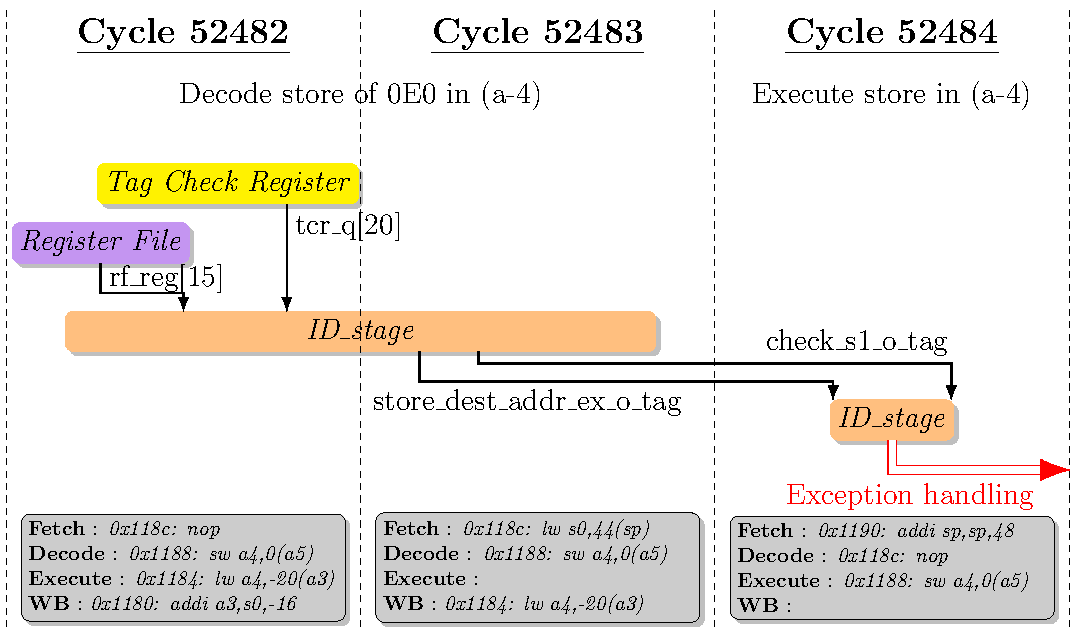
\includegraphics[height=.85\textheight]{src/2_vuln_assessment/img/wuftpd/ftpd_short.pdf}
        \caption{Temporal analysis of the tags propagation in a \textit{format string} attack}
        \label{fig:analyseTempoFormatString}
    \end{figure}
\end{frame}

\begin{frame}
    \begin{figure}
        \centering
        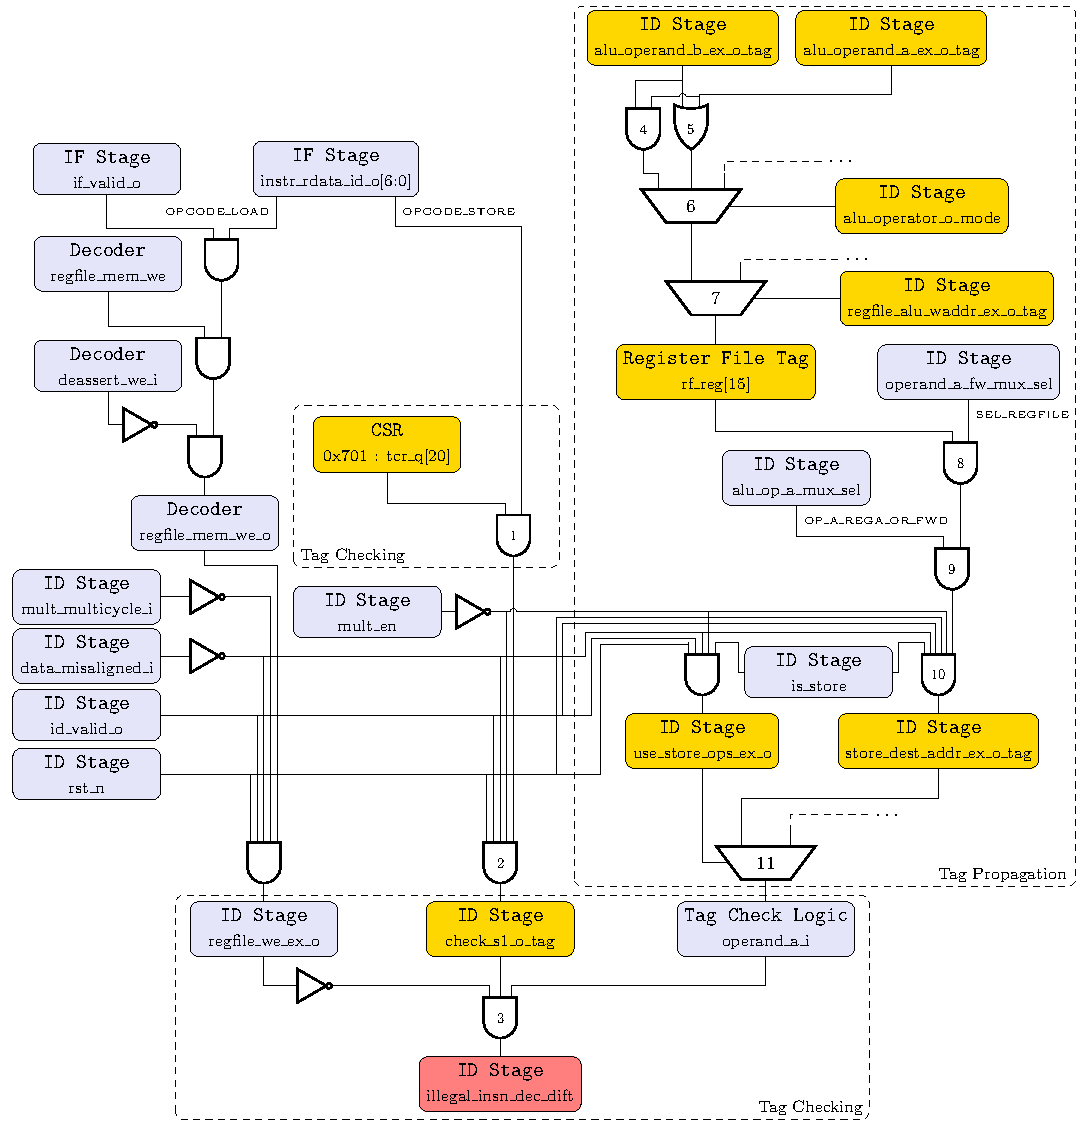
\includegraphics[height=.85\textheight]{src/2_vuln_assessment/img/wuftpd/arborescence_wuftpd.pdf}
        \caption{Logical analysis of the tags propagation in a \textit{format string} attack}
        \label{fig:analyseLogiqueFormatString}
    \end{figure}
\end{frame}
%%%%%%%%%%%%%%%%%%%%%%%%%%%%%%%%%%%%%%%%%%%%%%%%%%%%%%%%%%%%%%%%%%%%%%%%%%%%%%%%%%%%%%%%%%%%%%%%%%%%%%%%%%%%
\subsection{Experimental Setup}
%%%%%%%%%%%%%%%%%%%%%%%%%%%%%%%%%%%%%%%%%%%%%%%%%%%%%%%%%%%%%%%%%%%%%%%%%%%%%%%%%%%%%%%%%%%%%%%%%%%%%%%%%%%%
\begin{frame}{Experimental Setup - Simulation fault injections campaign}
    \begin{itemize}
        \justifying
        \item Logical fault injection simulation is used for preliminary evaluations
              \begin{itemize}
                  \justifying
                  \item faults are injected in the HDL code at cycle accurate and bit accurate level
                  \item a set of 55 DIFT-related registers are targeted
                  \item a reference simulation is done without fault
                  \item results are classed in four groups
                        \begin{itemize}
                            \justifying
                            \item crash: reference cycle count exceeded,
                            \item silent: current faulted simulation is the same as the reference simulation
                            \item delay: illegal instruction is delayed
                            \item success: DIFT has been bypassed
                        \end{itemize}
              \end{itemize}
        \item Simulations with QuestaSim 10.6e.
    \end{itemize}
\end{frame}
%%%%%%%%%%%%%%%%%%%%%%%%%%%%%%%%%%%%%%%%%%%%%%%%%%%%%%%%%%%%%%%%%%%%%%%%%%%%%%%%%%%%%%%%%%%%%%%%%%%%%%%%%%%%
\begin{frame}{Main results : 3 cases}
    \begin{table}[H]
        \centering
        \caption{End of simulation status}
        \label{table:end_sim_by_status}
        \begin{tabular}{lrrrlr}
            \toprule
                            & Crash & NSTR & Delay & Success     & Total \\
            \midrule
            Buffer overflow & 0     & 1380 & 20    & 22 (1.55\%) & 1422  \\
            WU-FTPd         & 0     & 1767 & 77    & 52 (2.74\%) & 1896  \\
            Compare/Compute & 0     & 917  & 12    & 19 (2.00\%) & 948   \\
            \bottomrule
        \end{tabular}
    \end{table}
\end{frame}

\begin{frame}{Buffer overflow}
    \begin{table}[]
        \centering
        \caption{Buffer overflow : Register sensitivity as determined by fault model and simulation time}
        \label{table:end_sim_from_time_fault_register_buffer_overflow}
        \resizebox{\textwidth}{!}{%
            \begin{tabular}{llllllllllllllll}
                \toprule
                                                & \multicolumn{3}{c}{Cycle 3428} & \multicolumn{3}{c}{Cycle 3429} & \multicolumn{3}{c}{Cycle 3430} & \multicolumn{3}{c}{Cycle 3431} & \multicolumn{3}{c}{Cycle 3432}                                                                                                                 \\\cmidrule(lr){2-4}\cmidrule(lr){5-7}\cmidrule(lr){8-10}\cmidrule(lr){11-13}\cmidrule(lr){14-16}
                                                & set0                           & set1                           & bitflip                        & set0                           & set1                           & bitflip    & set0       & set1 & bitflip    & set0       & set1 & bitflip    & set0       & set1 & bitflip    \\
                \midrule
                pc\_if\_o\_tag                  &                                &                                &                                &                                &                                &            &            &      &            & \checkmark &      & \checkmark &            &      &            \\
                rf\_reg[1]                      &                                &                                &                                &                                &                                &            & \checkmark &      & \checkmark &            &      &            &            &      &            \\
                tcr\_q                          & \checkmark                     &                                &                                & \checkmark                     &                                &            & \checkmark &      &            & \checkmark &      &            & \checkmark &      &            \\
                \rowcolor{LightGray} tcr\_q[21] &                                &                                & \checkmark                     &                                &                                & \checkmark &            &      & \checkmark &            &      & \checkmark &            &      & \checkmark \\
                tpr\_q                          & \checkmark                     & \checkmark                     &                                & \checkmark                     & \checkmark                     &            &            &      &            &            &      &            &            &      &            \\
                \rowcolor{LightGray} tpr\_q[12] &                                &                                & \checkmark                     &                                &                                & \checkmark &            &      &            &            &      &            &            &      &            \\
                \rowcolor{LightGray} tpr\_q[15] &                                &                                & \checkmark                     &                                &                                & \checkmark &            &      &            &            &      &            &            &      &            \\
                \bottomrule
            \end{tabular}
        }
    \end{table}
\end{frame}

\begin{frame}{Discussion}
    \begin{itemize}
        \setbeamertemplate{itemize items}[triangle]
        \item 4212 simulations have been performed,
        \item 93 successes (2.21\%),
        \item We have shown that the D-RI5CY DIFT is vulnerable to FIA
        \item Propagation of faults is facilitated by paths fully made of \textit{AND} gates
    \end{itemize}
\end{frame}
%%%%%%%%%%%%%%%%%%%%%%%%%%%%%%%%%%%%%%%%%%%%%%%%%%%%%%%%%%%%%%%%%%%%%%%%%%%%%%%%%%%%%%%%%%%%%%%%%%%%%%%%%%%%
%
% ---------------------------------------------------------------- %
\section{Fault Injection Simulation for Security Assessment}

\begin{frame}{FISSA - Fault Injection Simulation for Security Assessment}
    \begin{itemize}
        \item quelques mots sur l'outil
        \item parler à la première du singulier
        \item images d'Architecture
        \item lien github
        \item citation vers articles
        \item aller vite vers résultat (pas d'exemples, trop long ...)
    \end{itemize}
\end{frame}
%
% ---------------------------------------------------------------- %
\section{Solutions to Protect against FIAs}

%%%%%%%%%%%%%%%%%%%%%%%%%%%%%%%%%%%%%%%%%%%%%%%%%%%%%%%%%%%%%%%%%%%%%%%%%%%%%%%%%%%%%%%%%%%%%%%%%%%%%%%%%%%%
\begin{frame}{Introduction}
    \begin{block}{Protections}
        \begin{itemize}
            \item Focusing on lightweight hardware countermeasures:
            \begin{itemize}
                \item \textbf{Hardware redundancy}: duplication, or triplication, of the circuit to compare the results obtained to check for any difference;
                \item \textbf{Temporal redundancy}: repeating operations in reverse to compare the result with the initial value;
                \item \textbf{Instruction replay}: executing multiple times the same instruction or block of instructions;
                \item \textbf{Obfuscation}: addition of dummy cycles, or shuffle the data;
                \only<1>{\item \textbf{Information redundancy}: adding additional data to the information to detect or correct the initial value, such as simple parity code, Hamming Code, BCH code, or Reed-Solomon.}
                \only<2>{\item \textcolor{red}{\textbf{Information redundancy}: adding additional data to the information to detect or correct the initial value, such as simple parity code, Hamming Code, BCH code, or Reed-Solomon.}}
            \end{itemize}
        \end{itemize}
    \end{block}

    \note{lightweight : only add a few bits of data without an overhead on performances to detect and correct 1 or 2 errors}
\end{frame}
%%%%%%%%%%%%%%%%%%%%%%%%%%%%%%%%%%%%%%%%%%%%%%%%%%%%%%%%%%%%%%%%%%%%%%%%%%%%%%%%%%%%%%%%%%%%%%%%%%%%%%%%%%%%
\begin{frame}{Countermeasures}
    \begin{block}{Protections}
        \begin{itemize}
            \item Focusing on information redundancy codes:
            \begin{itemize}
                \item Simple parity
                \item Hamming Code
                \item Hamming Code with an additional bit (SECDED)
            \end{itemize}
            \item Implementations of \textit{Hamming Code} and \textit{Simple parity} have been presented at ISVLSI 2024~\cite{PRLG-24-isvlsi}.
        \end{itemize}
    \end{block}
\end{frame}
%%%%%%%%%%%%%%%%%%%%%%%%%%%%%%%%%%%%%%%%%%%%%%%%%%%%%%%%%%%%%%%%%%%%%%%%%%%%%%%%%%%%%%%%%%%%%%%%%%%%%%%%%%%%
\subsection{Simple Parity}
    \begin{frame}{Detection of single-bit errors — Simple Parity}
        \begin{block}{}
            \begin{itemize}
                \justifying
                \item Often used for error detection.
                \item Add an extra bit for parity computation.
                \item Can only detect one error without correction.
            \end{itemize}
        \end{block}

        \vfill
        
        \begin{figure}
            \centering
            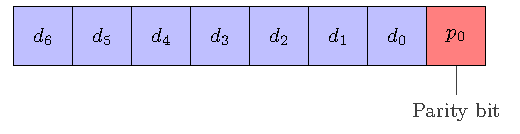
\includegraphics[width=.5\textwidth, page=1]{src/4_strategies/img/simple_parity.pdf}
            \caption{Simple parity codeword}
            \label{fig:simple_parity_codeword}
        \end{figure}
    \end{frame}
%%%%%%%%%%%%%%%%%%%%%%%%%%%%%%%%%%%%%%%%%%%%%%%%%%%%%%%%%%%%%%%%%%%%%%%%%%%%%%%%%%%%%%%%%%%%%%%%%%%%%%%%%%%%
\subsection{Hamming Code}
    \begin{frame}{Detection and correction of single-bit errors — Hamming Code}
        \begin{block}{}
            \begin{itemize}
                \justifying
                \item Linear error-correcting codes, invented by Richard W. Hamming~\cite{H-50-bstj}.
                \item Mostly used in digital communication and data storage systems.
                \item Detect and correct single-bit error.
                \item Redundancy bits are placed in power of 2 positions.
                % \item The number of redundancy bits depends on the number of bits to be protected {\scriptsize ($ 2^r \ge m + r + 1 $)}
            \end{itemize}
        \end{block}

        \begin{minipage}[c]{0.4\linewidth}
            \begin{equation} \label{equat:hamming_encoder}
                \begin{split}
                    r_{0} &= d_{0} \oplus d_{1} \oplus d_{3} \oplus d_{4} \oplus d_{6} \\
                    r_{1} &= d_{0} \oplus d_{2} \oplus d_{3} \oplus d_{5} \oplus d_{6} \\
                    r_{2} &= d_{1} \oplus d_{2} \oplus d_{3} \\
                    r_{3} &= d_{4} \oplus d_{5} \oplus d_{6}
                \end{split}
            \end{equation}
        \end{minipage}\hfill%
        \begin{minipage}[c]{0.55\linewidth}
            \begin{figure}
                \centering
                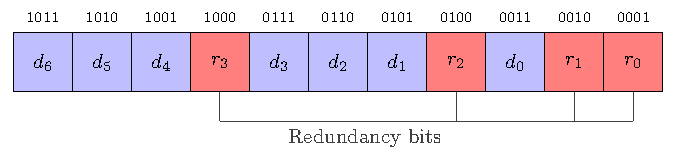
\includegraphics[width=\textwidth, page=1]{src/4_strategies/img/hamming_bit.pdf}
                \caption{Hamming codeword}
                \label{fig:hamming_codeword}
            \end{figure}
        \end{minipage}
    \end{frame}
%%%%%%%%%%%%%%%%%%%%%%%%%%%%%%%%%%%%%%%%%%%%%%%%%%%%%%%%%%%%%%%%%%%%%%%%%%%%%%%%%%%%%%%%%%%%%%%%%%%%%%%%%%%%
\subsection{Hamming Code — SECDED}
\begin{frame}{Detection of two-bit errors and correction of single-bit errors — SECDED}
    \begin{block}{}
        \begin{itemize}
            \justifying
            \item Based on Hamming Code.
            \item Detect two-bit error and correct single-bit error.
            \item An additional bit is added: general parity bit
        \end{itemize}
    \end{block}

    \begin{minipage}[c]{0.4\linewidth}
        \begin{equation} \label{equat:secded_encoder}
            \begin{split}
                r_{0}  &= d_{0} \oplus d_{1} \oplus d_{3} \oplus d_{4} \oplus d_{6} \\
                r_{1}  &= d_{0} \oplus d_{2} \oplus d_{3} \oplus d_{5} \oplus d_{6} \\
                r_{2}  &= d_{1} \oplus d_{2} \oplus d_{3} \\
                r_{3}  &= d_{4} \oplus d_{5} \oplus d_{6} \\
                gp_{0} &= \bigoplus_{i=0}^{6} d_{i} \oplus \bigoplus_{j=0}^{3} r_{j}
            \end{split}
        \end{equation}
    \end{minipage}\hfill%
    \begin{minipage}[c]{0.6\linewidth}
        \begin{figure}
            \centering
            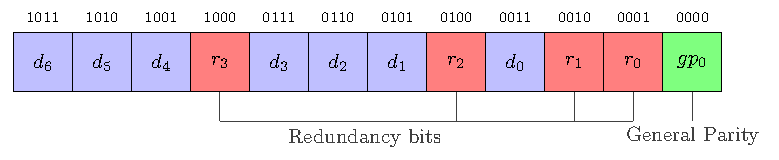
\includegraphics[width=\textwidth, page=1]{src/4_strategies/img/secded.pdf}
            \caption{SECDED codeword}
            \label{fig:secded_codeword}
        \end{figure}
    \end{minipage}
\end{frame}
%%%%%%%%%%%%%%%%%%%%%%%%%%%%%%%%%%%%%%%%%%%%%%%%%%%%%%%%%%%%%%%%%%%%%%%%%%%%%%%%%%%%%%%%%%%%%%%%%%%%%%%%%%%%
\begin{frame}{Implementation — One register for one encoder}
    \begin{figure}
        \centering
        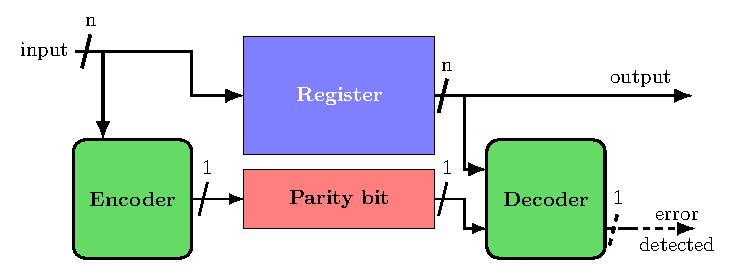
\includegraphics[width=.75\textwidth, page=1]{src/4_strategies/img/archi_contremesures.pdf}
        \caption{Implementation of a protection for one register}
        \label{fig:simple_parity_implem}
    \end{figure}
\end{frame}

\begin{frame}{Implementation — Multiple registers for one encoder}
    \begin{figure}
        \centering
        \includegraphics[width=.8\textwidth, page=4]{src/4_strategies/img/archi_contremesures.pdf}
        \caption{Implementation of a protection for multiple registers}
        \label{fig:secded_implem_independant_register}
    \end{figure}
\end{frame}

\begin{frame}{Implementation — One register on multiple encoders}
    \begin{figure}
        \centering
        \includegraphics[width=.9\textwidth, page=6]{src/4_strategies/img/archi_contremesures.pdf}
        \caption{Implementation of a protection for one register split}
        \label{fig:secded_implem_splitted}
    \end{figure}
\end{frame}

\begin{frame}{Implementation — Special case for Register File tag}
    \begin{figure}
        \centering
        \includegraphics[width=.9\textwidth, page=5]{src/4_strategies/img/archi_contremesures.pdf}
        \caption{Special implementation for the Register File Tag}
        \label{fig:secded_implem_rf}
    \end{figure}
\end{frame}
%%%%%%%%%%%%%%%%%%%%%%%%%%%%%%%%%%%%%%%%%%%%%%%%%%%%%%%%%%%%%%%%%%%%%%%%%%%%%%%%%%%%%%%%%%%%%%%%%%%%%%%%%%%%
\begin{frame}{Implemented strategies — Evaluation of Group Composition}
    \begin{block}{}
        \begin{itemize}
            \justifying
            \item Different strategies of implementation can be done depending on the objective
            \item The protection efficiency would vary
            \item We want the best protection at the lowest cost possible against different fault models
        \end{itemize}
    \end{block}
\end{frame}

\begin{frame}{Implemented strategies — Group composition}
    \begin{table}[t]
        \centering
        \small
        \caption{Grouping composition and objectives of implemented strategies}
        \label{tab:strategies_group}
        % \setlength{\tabcolsep}{2pt}
        \begin{tabular}{@{}cm{4cm}m{7cm}@{}}
            \toprule
                                & \tableCentered{Grouping strategy}           & Objective                                                       \\ \midrule
            Strategy 1          & Minimisation of groups                      & Minimisation of the area overhead                               \\
            Strategy 2          & Protection per pipeline stage               & One protection for each 7 pipeline stages                       \\
            Strategy 3          & Protection per register                     & Each register is protected individually                         \\
            Strategy 4          & Protection per register with CSR splitting  & Strategy 3 + Split the CSRs registers by group of operations    \\
            Strategy 5          & Coupling split registers                    & Split each register and couple each bit to another register     \\
            \bottomrule
        \end{tabular}
    \end{table}
\end{frame}
%%%%%%%%%%%%%%%%%%%%%%%%%%%%%%%%%%%%%%%%%%%%%%%%%%%%%%%%%%%%%%%%%%%%%%%%%%%%%%%%%%%%%%%%%%%%%%%%%%%%%%%%%%%%
\begin{frame}{Implemented strategies — details}
    \begin{figure}
        \centering
        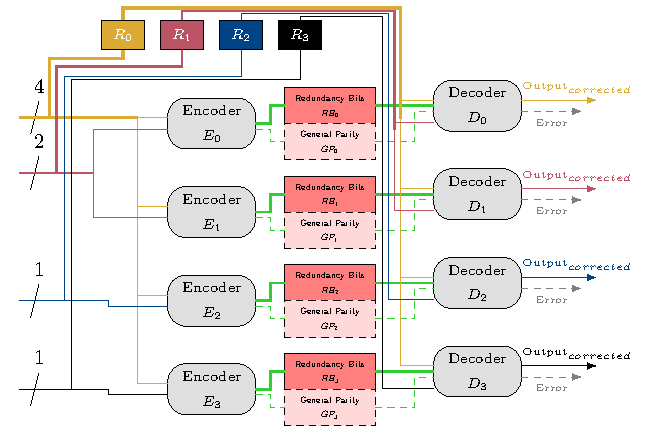
\includegraphics[height=.8\textheight]{src/4_strategies/img/implem5_spaghetti.pdf}
        \caption{Representation of the fifth strategy}
        \label{fig:strategy_5}
    \end{figure}
\end{frame}
%%%%%%%%%%%%%%%%%%%%%%%%%%%%%%%%%%%%%%%%%%%%%%%%%%%%%%%%%%%%%%%%%%%%%%%%%%%%%%%%%%%%%%%%%%%%%%%%%%%%%%%%%%%%
%
% ---------------------------------------------------------------- %
\section{Experimental results}

%%%%%%%%%%%%%%%%%%%%%%%%%%%%%%%%%%%%%%%%%%%%%%%%%%%%%%%%%%%%%%%%%%%%%%%%%%%%
\begin{frame}{Experimental setup}
    \begin{minipage}[c]{0.7\linewidth}
        \begin{block}{}
            \begin{itemize}
                \item Use of FISSA for FIA campaigns
                \item More complex fault models: multi-bit faults or multi single-bit faults
            \end{itemize}
        \end{block}
    \end{minipage}\hfill%
    \begin{minipage}[c]{0.3\linewidth}
        \begin{figure}
            \centering
            
\includegraphics[width=.75\textwidth]{src/5_results/img/experimental.png}
        \end{figure}
    \end{minipage}
\end{frame}
%%%%%%%%%%%%%%%%%%%%%%%%%%%%%%%%%%%%%%%%%%%%%%%%%%%%%%%%%%%%%%%%%%%%%%%%%%%%
\begin{frame}{Fault model}
    \begin{block}{}
        \begin{itemize}
            \item DIFT-related registers + protection-related registers
            \item Single bit-flip in two registers at two distinct clock cycles {\footnotesize$\Rightarrow$ 1 bit faulted per clock cycle}
            \item \underline{Single bit-flip in two registers at a given clock cycle} {\footnotesize$\Rightarrow$ 2 bits faulted per clock cycle}
            \item Multi-bit faults in one register at a given clock cycle {\footnotesize$\Rightarrow$ up to 6 bits faulted per clock cycle} {\tiny (registers from 1 to 10 bits only)}
            \item \underline{Multi-bit faults in two registers at a given clock cycle} {\footnotesize$\Rightarrow$ up to 11 bits faulted per clock cycle} {\tiny (registers from 1 to 10 bits only)}
        \end{itemize}
    \end{block}
\end{frame}
%%%%%%%%%%%%%%%%%%%%%%%%%%%%%%%%%%%%%%%%%%%%%%%%%%%%%%%%%%%%%%%%%%%%%%%%%%%%%%%%%%%%%%%%%%%%%%%%%%%%%%%%%%%%
\begin{frame}{FPGA implementation results}
    \begin{table}[t]
        \centering
        \footnotesize
        \caption{FPGA implementation results\footnote{Zedboard Xilinx Zynq-7000} — Vivado 2023.2}
        \label{tab:chap6_implementation}
        \begin{tabular}{@{}rccc@{}}
            \toprule
            \tableCentered{Protection} & Number of LUTs                                     & Number of FFs                                      & Maximum frequency                        \\ \midrule
            D-RI5CY                    & \num{6911} {\tiny (0\%)   }                        & \num{2335} {\tiny (0\%)   }                        & \SI{47.6}{\mega\hertz} {\tiny (0\%)    } \\
            Simple parity              & \num{7011} {\tiny (+1.45\%)}                        & \num{2337} {\tiny (+0.09\%)}                        & \SI{47.6}{\mega\hertz} {\tiny (0\%)    } \\
            Hamming Code Strategy 1    & \num{7283} {\tiny (+5.38\%)}                        & \textcolor{LimeGreen}{\num{2361} {\tiny (+1.11\%)}} & \SI{47.4}{\mega\hertz} {\tiny (-0.36\%)} \\
            Hamming Code Strategy 2    & \textcolor{red}{\num{7369} {\tiny (+6.63\%)}}       & \num{2363} {\tiny (+1.2\%) }                        & \SI{46.9}{\mega\hertz} {\tiny (-1.43\%)} \\
            Hamming Code Strategy 3    & \num{7251} {\tiny (+4.92\%)}                        & \num{2361} {\tiny (+1.11\%)}                        & \SI{46.8}{\mega\hertz} {\tiny (-1.67\%)} \\
            Hamming Code Strategy 4    & \num{7203} {\tiny (+4.23\%)}                        & \num{2371} {\tiny (+1.54\%)}                        & \SI{47.6}{\mega\hertz} {\tiny (0\%)    } \\
            Hamming Code Strategy 5    & \textcolor{LimeGreen}{\num{7182} {\tiny (+3.92\%)}} & \textcolor{red}{\num{2411} {\tiny (+3.25\%)}}       & \SI{47.3}{\mega\hertz} {\tiny (-0.57\%)} \\
            SECDED Strategy 1          & \num{7428} {\tiny (+7.48\%)}                        & \num{2366} {\tiny (+1.33\%)}                        & \SI{47.2}{\mega\hertz} {\tiny (-0.95\%)} \\
            SECDED Strategy 2          & \textcolor{red}{\num{7433} {\tiny (+7.55\%)}}       & \num{2366} {\tiny (+1.41\%)}                        & \SI{47.2}{\mega\hertz} {\tiny (-0.95\%)} \\
            SECDED Strategy 3          & \num{7324} {\tiny (+5.98\%)}                        & \textcolor{LimeGreen}{\num{2368} {\tiny (+1.28\%)}} & \SI{47.5}{\mega\hertz} {\tiny (-0.24\%)} \\
            SECDED Strategy 4          & \num{7255} {\tiny (+4.98\%)}                        & \num{2365} {\tiny (+1.93\%)}                        & \SI{48.3}{\mega\hertz} {\tiny (+1.43\%) } \\
            SECDED Strategy 5          & \textcolor{LimeGreen}{\num{7228} {\tiny (+4.59\%)}} & \textcolor{red}{\num{2428} {\tiny (+3.98\%)}}       & \SI{48.3}{\mega\hertz} {\tiny (+1.43\%) } \\
            \bottomrule
        \end{tabular}
    \end{table}
    
    \only<2>{
        \begin{columns}
            \begin{column}{.25\linewidth}
                \hfill
            \end{column}
            \begin{column}{.5\linewidth}
                \begin{alertblock}{}
                    \centering
                    \textcolor{red}{\Forward}~No major impact on area and performances~\textcolor{red}{\Rewind} 
                \end{alertblock}
            \end{column}
            \begin{column}{.25\linewidth}
                \hfill
            \end{column}
        \end{columns}
    }
    \note{FPGA rapidement : pas d'impacts}
\end{frame}
%%%%%%%%%%%%%%%%%%%%%%%%%%%%%%%%%%%%%%%%%%%%%%%%%%%%%%%%%%%%%%%%%%%%%%%%%%%%%%%%%%%%%%%%%%%%%%%%%%%%%%%%%%%%
\begin{frame}{Obtained results from the first considered fault model}
    \begin{table}[H]
        \scriptsize
        \centering
        \caption{Logical fault injection simulation campaigns results for single bit-flip in two registers at a given clock cycle}
        \label{tab:chap6_results_single_bitflip_spatial_bo}
        \setlength{\tabcolsep}{2pt}
        \begin{tabular}{@{}ccccccccccc@{}}
            \toprule
                                                               &               & Crash & Silent      & Delay      & Detection   & \tableTwoLines{Detection \&}{Correction} & \tableTwoLines{Double Error}{Detection} & Success                     & Total        & \tableTwoLines{Execution}{time (h:min)} \\\midrule
            \multirow{12}{*}{\tableTwoLines{Buffer}{Overflow}} & No protection & 0     & \num{45097} & \num{1503} & --          & --                                       & --                                      & \textcolor{blue}{\num{1406} {\tiny (2.93\%)}} & \textcolor{blue}{\num{48006}}  & 13:43                                   \\
                                                               & Simple parity & 0     & \num{10551} & 134        & \num{40952} & --                                       & --                                      & 239 {\tiny (0.46\%)}        & \num{51876 } & 14:07                                   \\
                                                               & Hamming 1     & 0     & 0           & 575        & --          & \num{67829 }                             & --                                      & \textcolor{red}{452 {\tiny (0.66\%)}}        & \textcolor{red}{\num{68856}} & 19:48                                   \\
                                                               & Hamming 2     & 0     & 0           & 297        & --          & \num{72867 }                             & --                                      & 312 {\tiny (0.42\%)}        & \num{73476 } & 97:16                                   \\
                                                               & Hamming 3     & 0     & 0           & 263        & --          & \num{108326}                             & --                                      & 281 {\tiny (0.26\%)}        & \num{108870} & 30:00                                   \\
                                                               & Hamming 4     & 0     & 0           & 57         & --          & \num{155112}                             & --                                      & 99  {\tiny (0.06\%)}        & \num{155268} & 46:30                                   \\
                                                               & Hamming 5     & 0     & 0           & 55         & --          & \num{173367}                             & --                                      & 98  {\tiny (0.06\%)}        & \num{173520} & 53:00                                   \\
                                                               & SECDED 1      & 0     & 2436        & 0          & --          & \num{59424 }                             & \num{11616}                             & \textcolor{LimeGreen}{0}                           & \textcolor{LimeGreen}{\num{73476 }} & 20:56                                   \\
                                                               & SECDED 2      & 0     & 0           & 0          & --          & \num{69354 }                             & \num{10842}                             & \textcolor{LimeGreen}{0}                           & \textcolor{LimeGreen}{\num{80196 }} & 21:49                                   \\
                                                               & SECDED 3      & 0     & 0           & 0          & --          & \num{128376}                             & \num{9654 }                             & \textcolor{LimeGreen}{0}                           & \textcolor{LimeGreen}{\num{138030}} & 40:14                                   \\
                                                               & SECDED 4      & 0     & 0           & 0          & --          & \num{204060}                             & \num{7410 }                             & \textcolor{LimeGreen}{0}                           & \textcolor{LimeGreen}{\num{211470}} & 64:02                                   \\
                                                               & SECDED 5      & 0     & \num{12096} & 0          & --          & \num{214722}                             & \num{7542 }                             & \textcolor{LimeGreen}{0}                           & \textcolor{LimeGreen}{\num{234360}} & 69:44                                   \\
            \bottomrule
        \end{tabular}
    \end{table}
\end{frame}

\begin{frame}{Obtained results from the second considered fault model}
    \begin{table}[H]
        \centering
        \footnotesize
        \caption{Logical fault injection simulation campaigns results for exhaustive multi-bits faults in two registers at a given clock cycle}
        \label{tab:chap6_results_multi_bitflip_reg_multi}
        \setlength{\tabcolsep}{2pt}
        \begin{tabular}{@{}ccccccccccc@{}}
            \toprule
                                                               &               & Crash & Silent       & Delay & Detection   & \tableTwoLines{Detection \&}{Correction} & \tableTwoLines{Double Error}{Detection} & Success                                      & Total        & \tableTwoLines{Execution}{time (h:min)} \\\midrule
            \multirow{12}{*}{\tableTwoLines{Buffer}{Overflow}} & No protection & 0     & \num{67072 } & 926   & --          & --                                       & --                                      & \textcolor{blue}{450 {\tiny (0.66\%)}}  & \textcolor{blue}{\num{68448}} & 11:11                                   \\
                                                               & Simple parity & 0     & \num{24622 } & 8     & \num{53359} & --                                       & --                                      & 59 {\tiny (0.08\%)}                          & \num{78048 } & 25:00                                   \\
                                                               & Hamming 1     & 0     & \num{294464} & 6273  & --          & --                                       & --                                      & 3103 {\tiny (1.02\%)}                        & \num{303840} & 99:36                                   \\
                                                               & Hamming 2     & 0     & 0            & 3992  & --          & \num{319588}                             & --                                      & \textcolor{red}{4356 {\tiny (1.33\%)}} & \textcolor{red}{\num{327936}} & 131:12                                  \\
                                                               & Hamming 3     & 0     & 0            & 4557  & --          & \num{436187}                             & --                                      & 4408 {\tiny (0.99\%)}                        & \num{445152} & 121:20                                  \\
                                                               & Hamming 4     & 0     & 0            & 5446  & --          & \num{590953}                             & --                                      & 5329 {\tiny (0.89\%)}                        & \num{601728} & 167:00                                  \\
                                                               & Hamming 5     & 0     & 0            & 5987  & --          & \num{714873}                             & --                                      & 5860 {\tiny (0.81\%)}                        & \num{726720} & 210:31                                  \\
                                                               & SECDED 1      & 0     & 0            & 1911  & --          & \num{150791}                             & \num{170575}                            & 723 {\tiny (0.22\%)}                         & \num{324000} & 86:59                                   \\
                                                               & SECDED 2      & 0     & 0            & 1186  & --          & \num{170805}                             & \num{184761}                            & 584 {\tiny (0.16\%)}                         & \num{357336} & 94:04                                   \\
                                                               & SECDED 3      & 0     & 0            & 1230  & --          & \num{300260}                             & \num{263665}                            & 669 {\tiny (0.12\%)}                         & \num{565824} & 161:30                                  \\
                                                               & SECDED 4      & 0     & 0            & 18    & --          & \num{457498}                             & \num{368959}                            & 61 {\tiny (0.0074\%)}                          & \num{826536} & 244:48                                  \\
                                                               & SECDED 5      & 0     & 0            & 39    & --          & \num{576992}                             & \num{401407}                            & \textcolor{LimeGreen}{66 {\tiny (0.0067\%)}}   & \textcolor{LimeGreen}{\num{978504}} & 284:45                                  \\
            \bottomrule
        \end{tabular}
    \end{table}
\end{frame}
%%%%%%%%%%%%%%%%%%%%%%%%%%%%%%%%%%%%%%%%%%%%%%%%%%%%%%%%%%%%%%%%%%%%%%%%%%%%%%%%%%%%%%%%%%%%%%%%%%%%%%%%%%%%
\begin{frame}{Generated heatmaps from FISSA with the current fault model}
    \begin{figure}
        \centering
        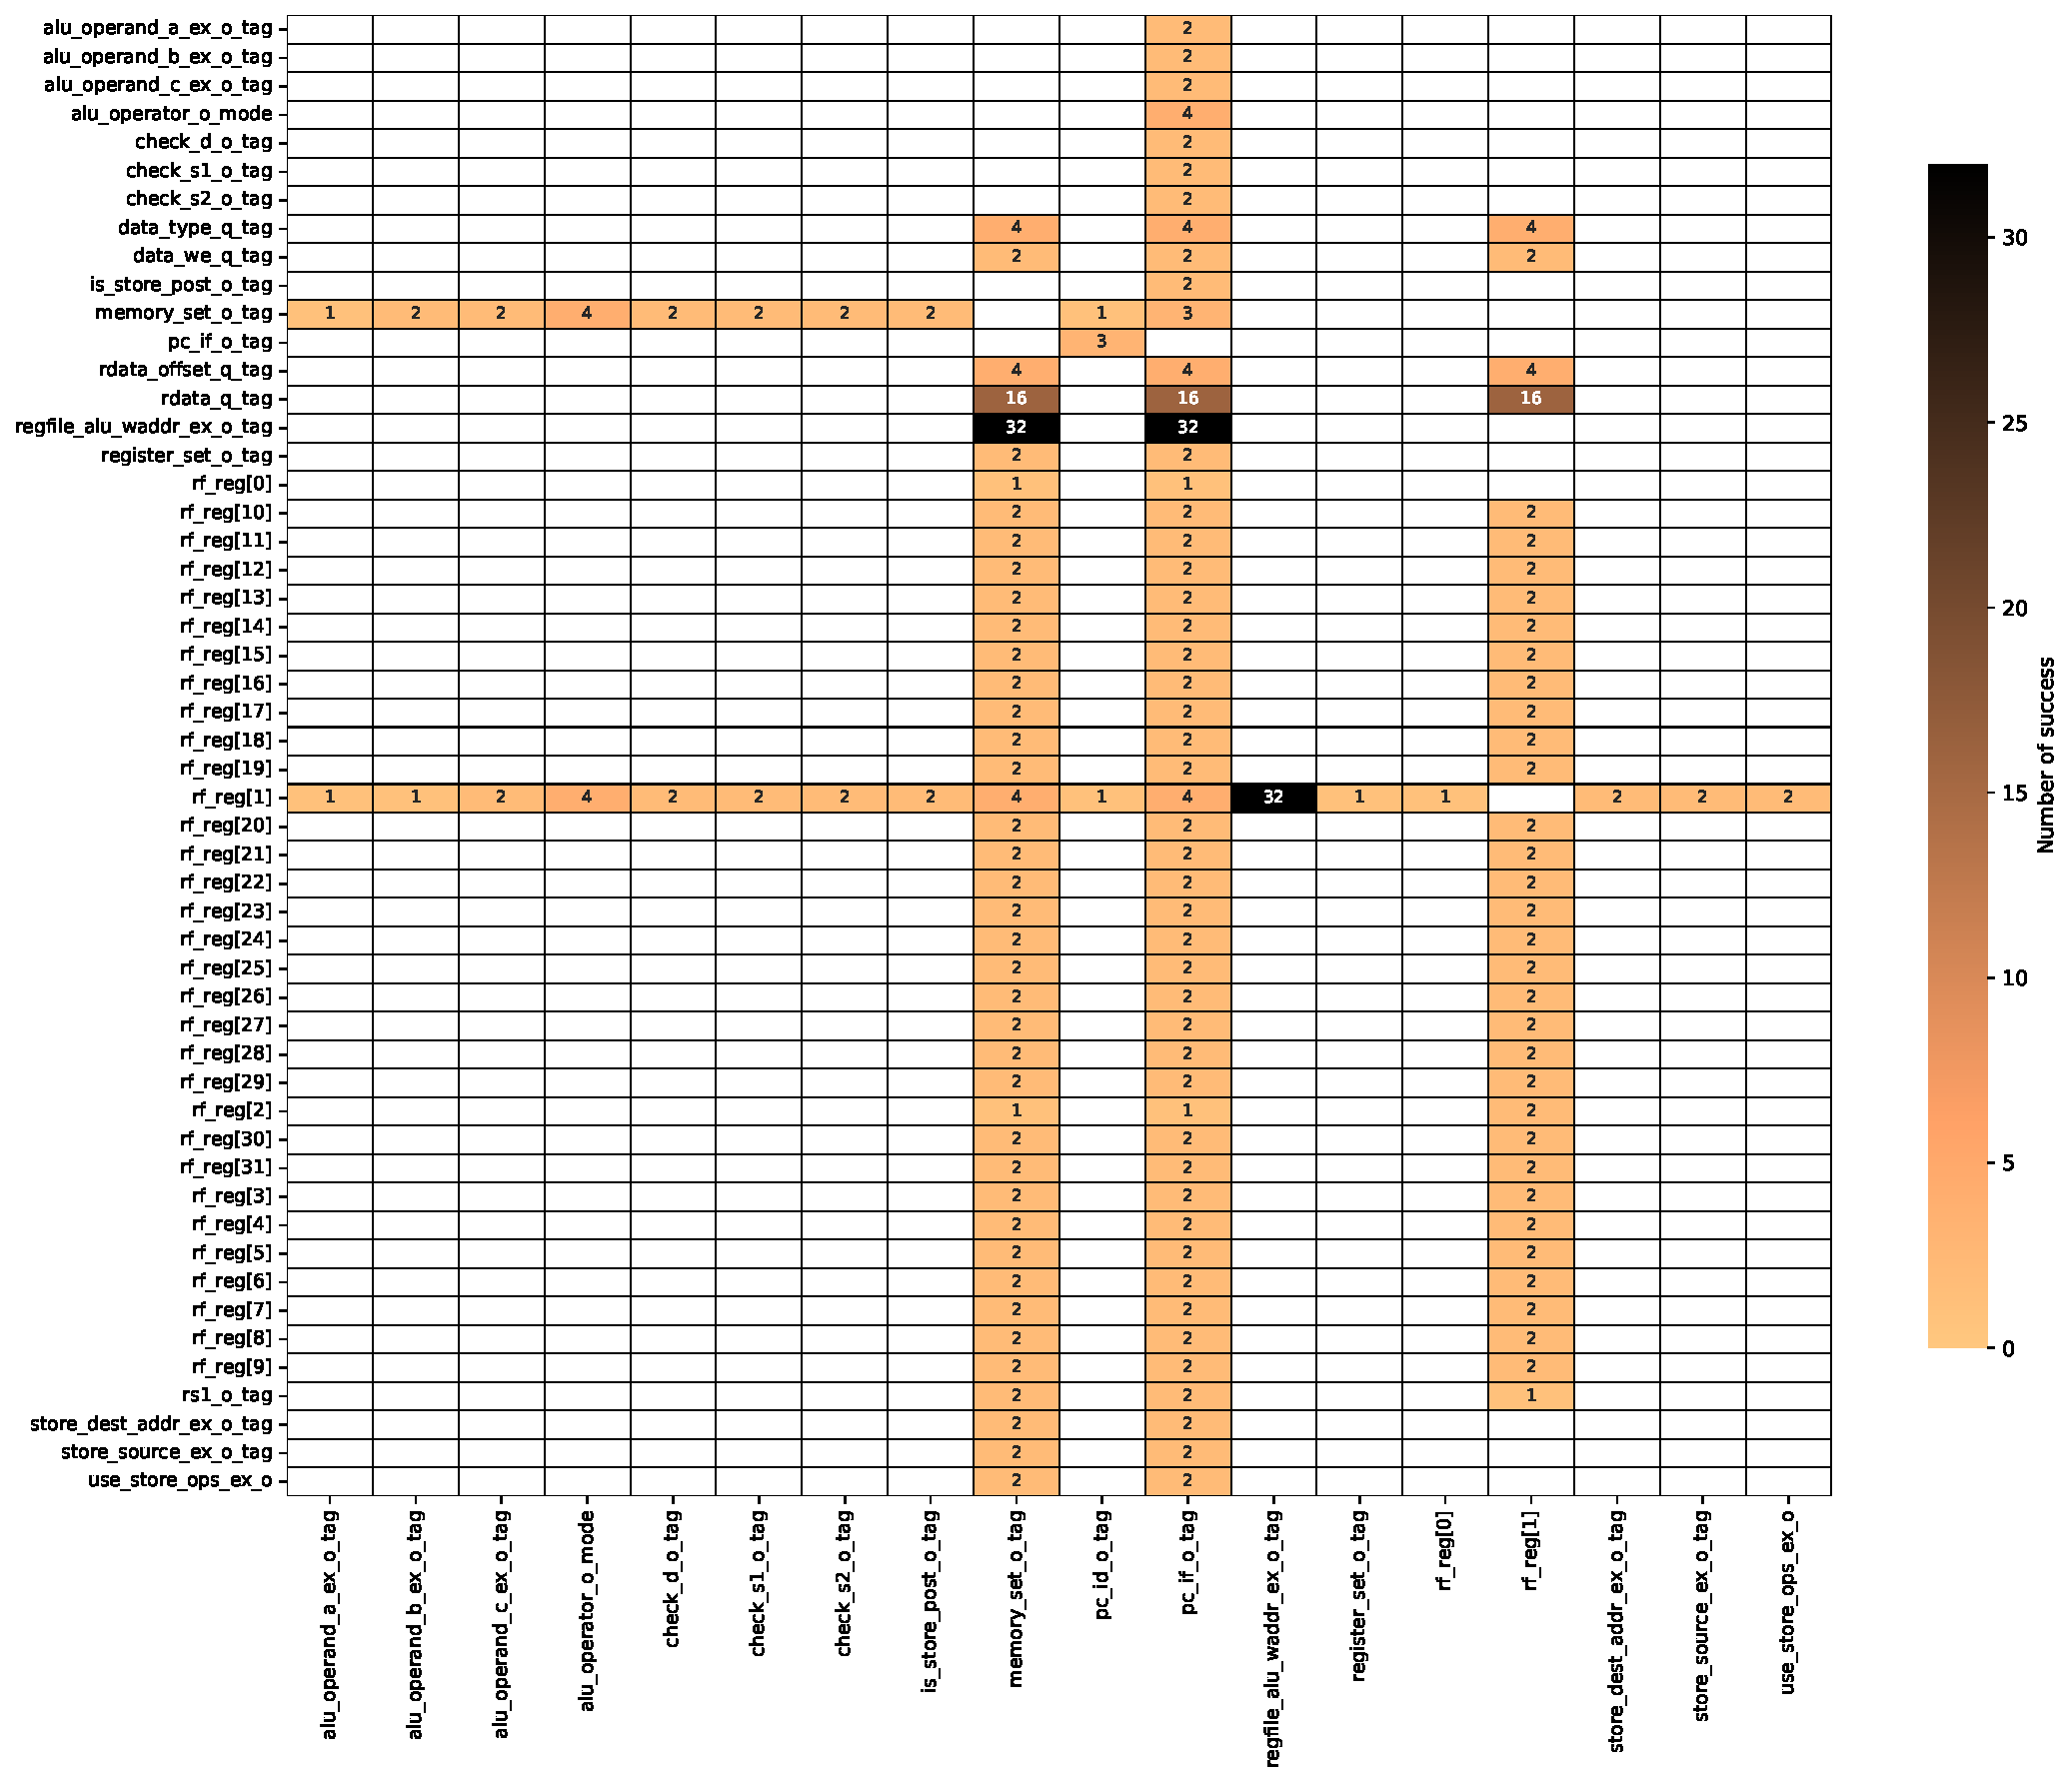
\includegraphics[height=.825\textheight]{src/5_results/img/heatmap_buffer_overflow_wop_1_multi_bitflip_reg_multi_2.pdf}
        \caption{Unprotected version: multi-bits faults in two registers at a given clock cycle $\rightarrow$ 450 successes}
        \label{fig:heatmap_multibit_0}
    \end{figure}
\end{frame}

\begin{frame}{}
    \begin{minipage}[c]{0.45\linewidth}
        \begin{figure}
            \centering
            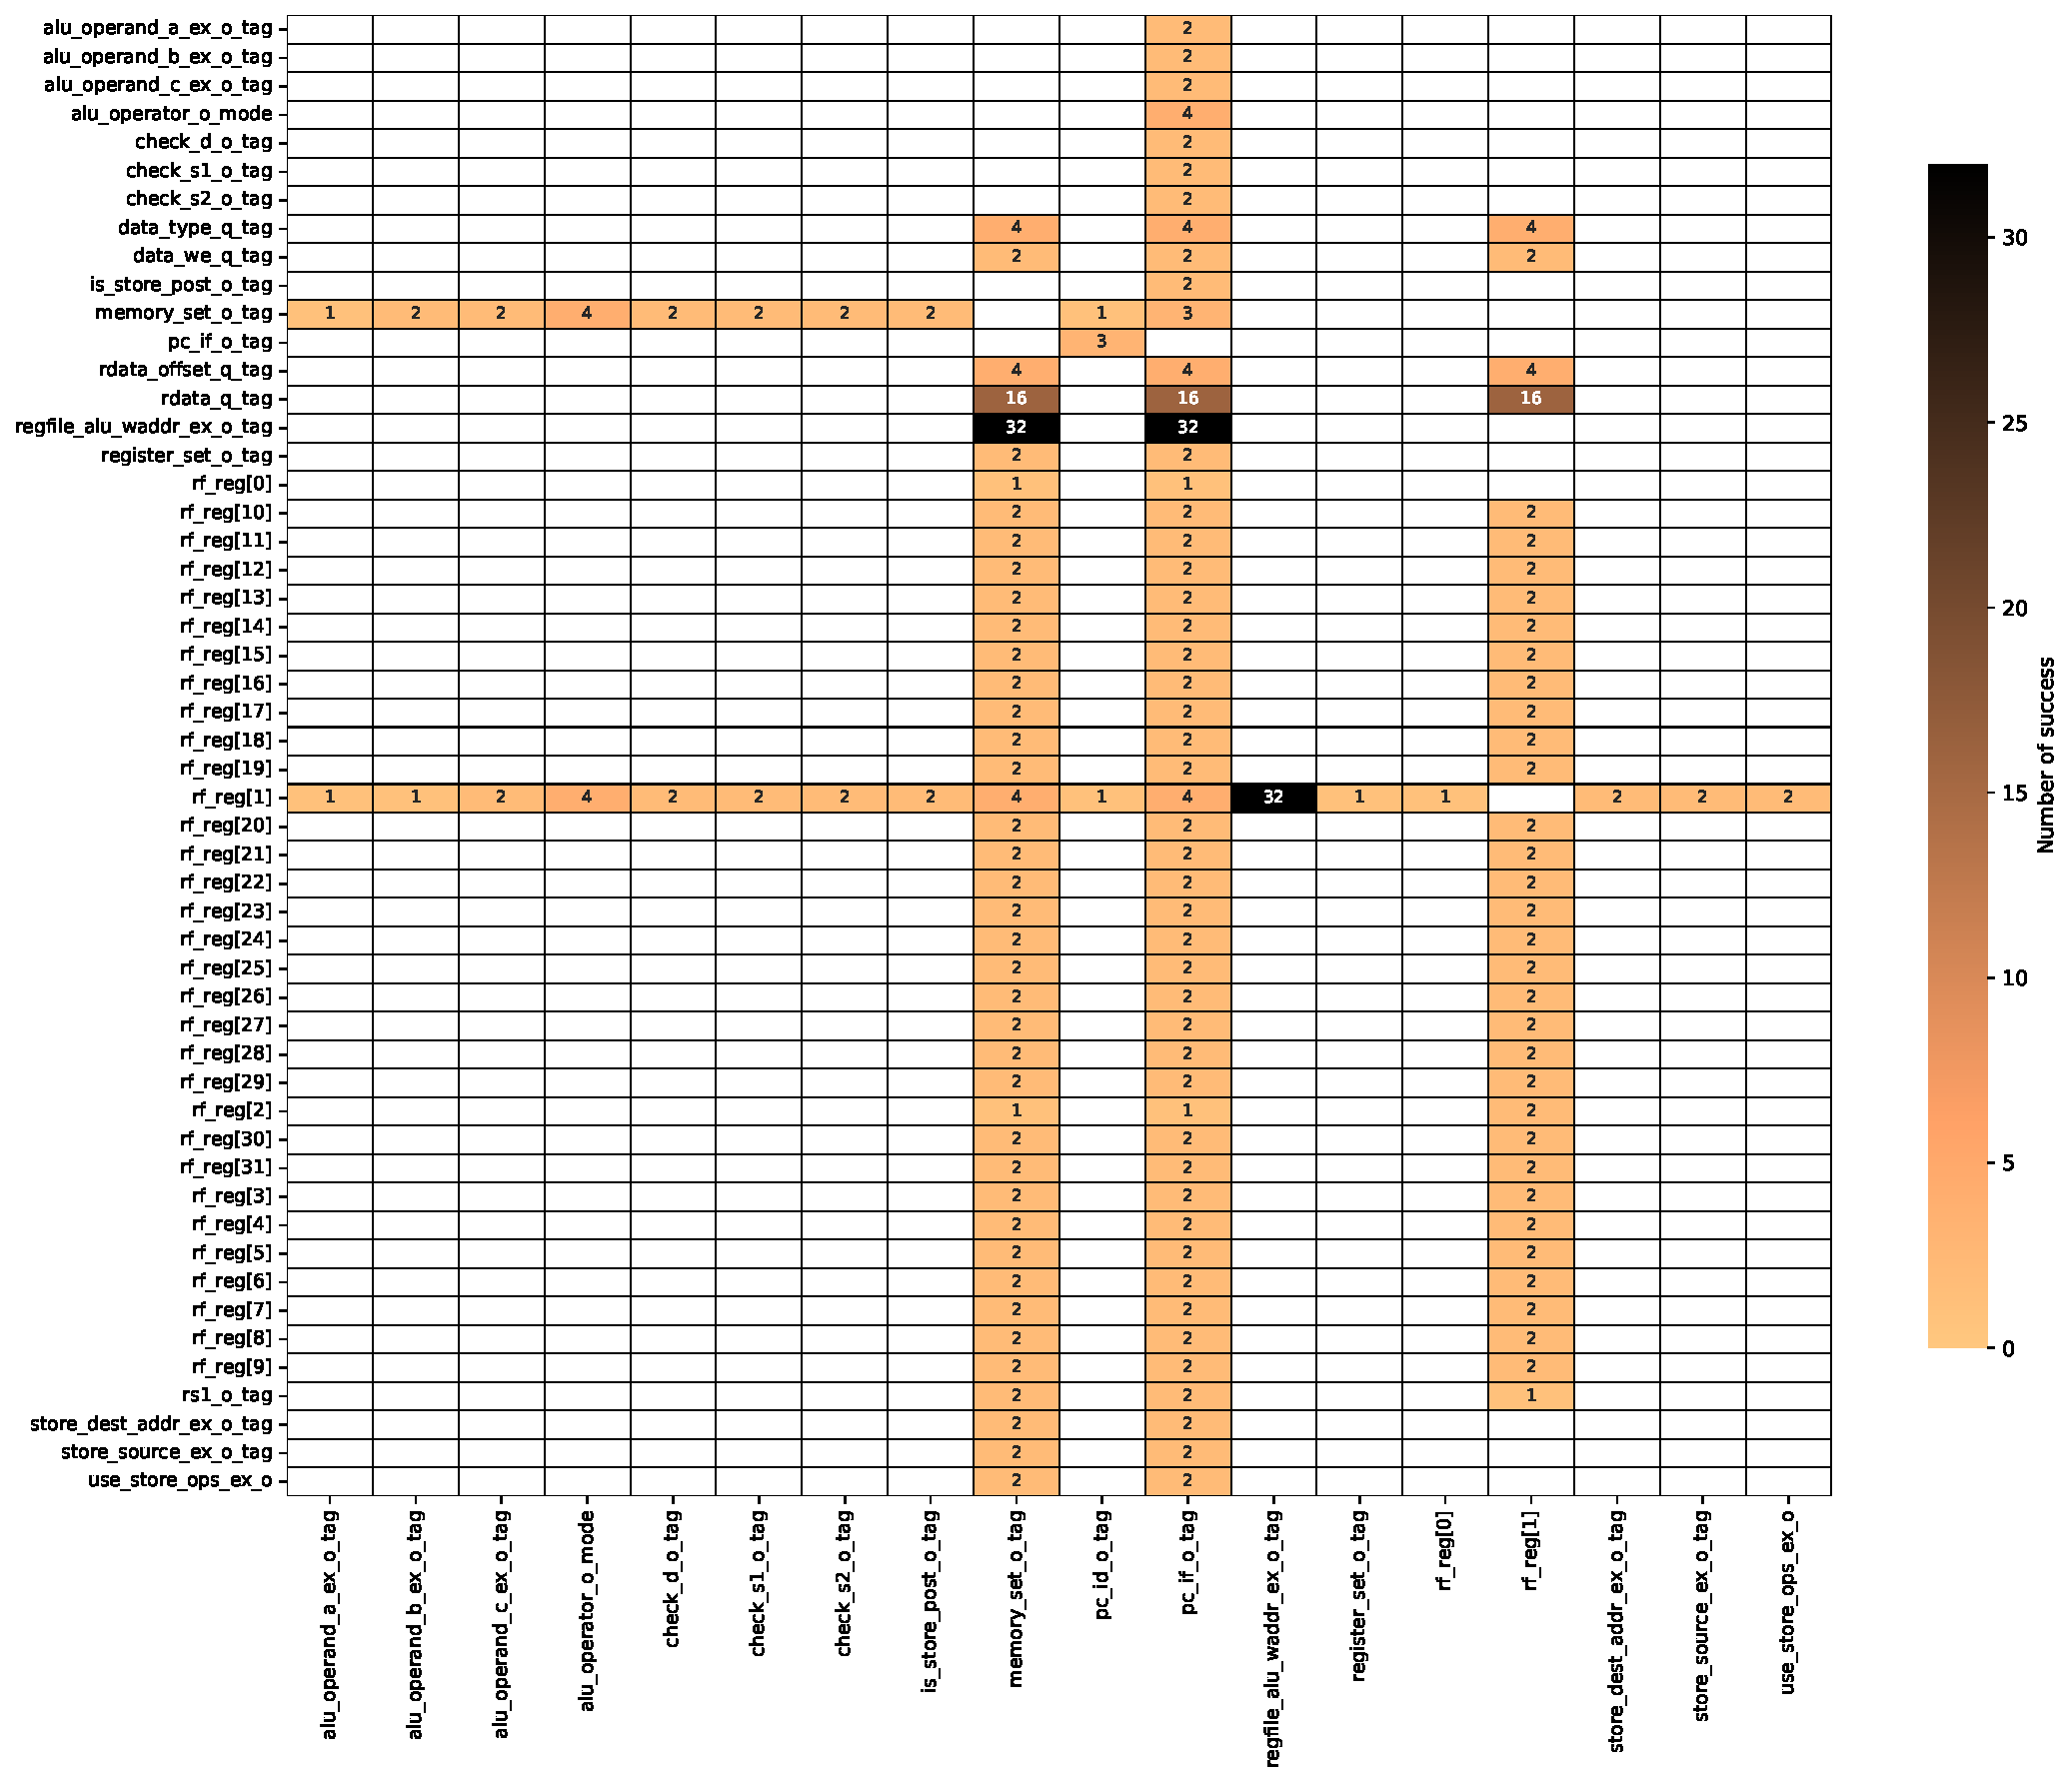
\includegraphics[width=\textwidth]{src/5_results/img/heatmap_buffer_overflow_wop_1_multi_bitflip_reg_multi_2.pdf}
            \caption{Unprotected version: multi-bits faults in two registers at a given clock cycle $\rightarrow$ 450 successes}
            \label{fig:heatmap_multibit_1}
        \end{figure}
    \end{minipage}\hfill%
    \begin{minipage}[c]{0.55\linewidth}
        \only<1>{
            \begin{figure}
                \centering
                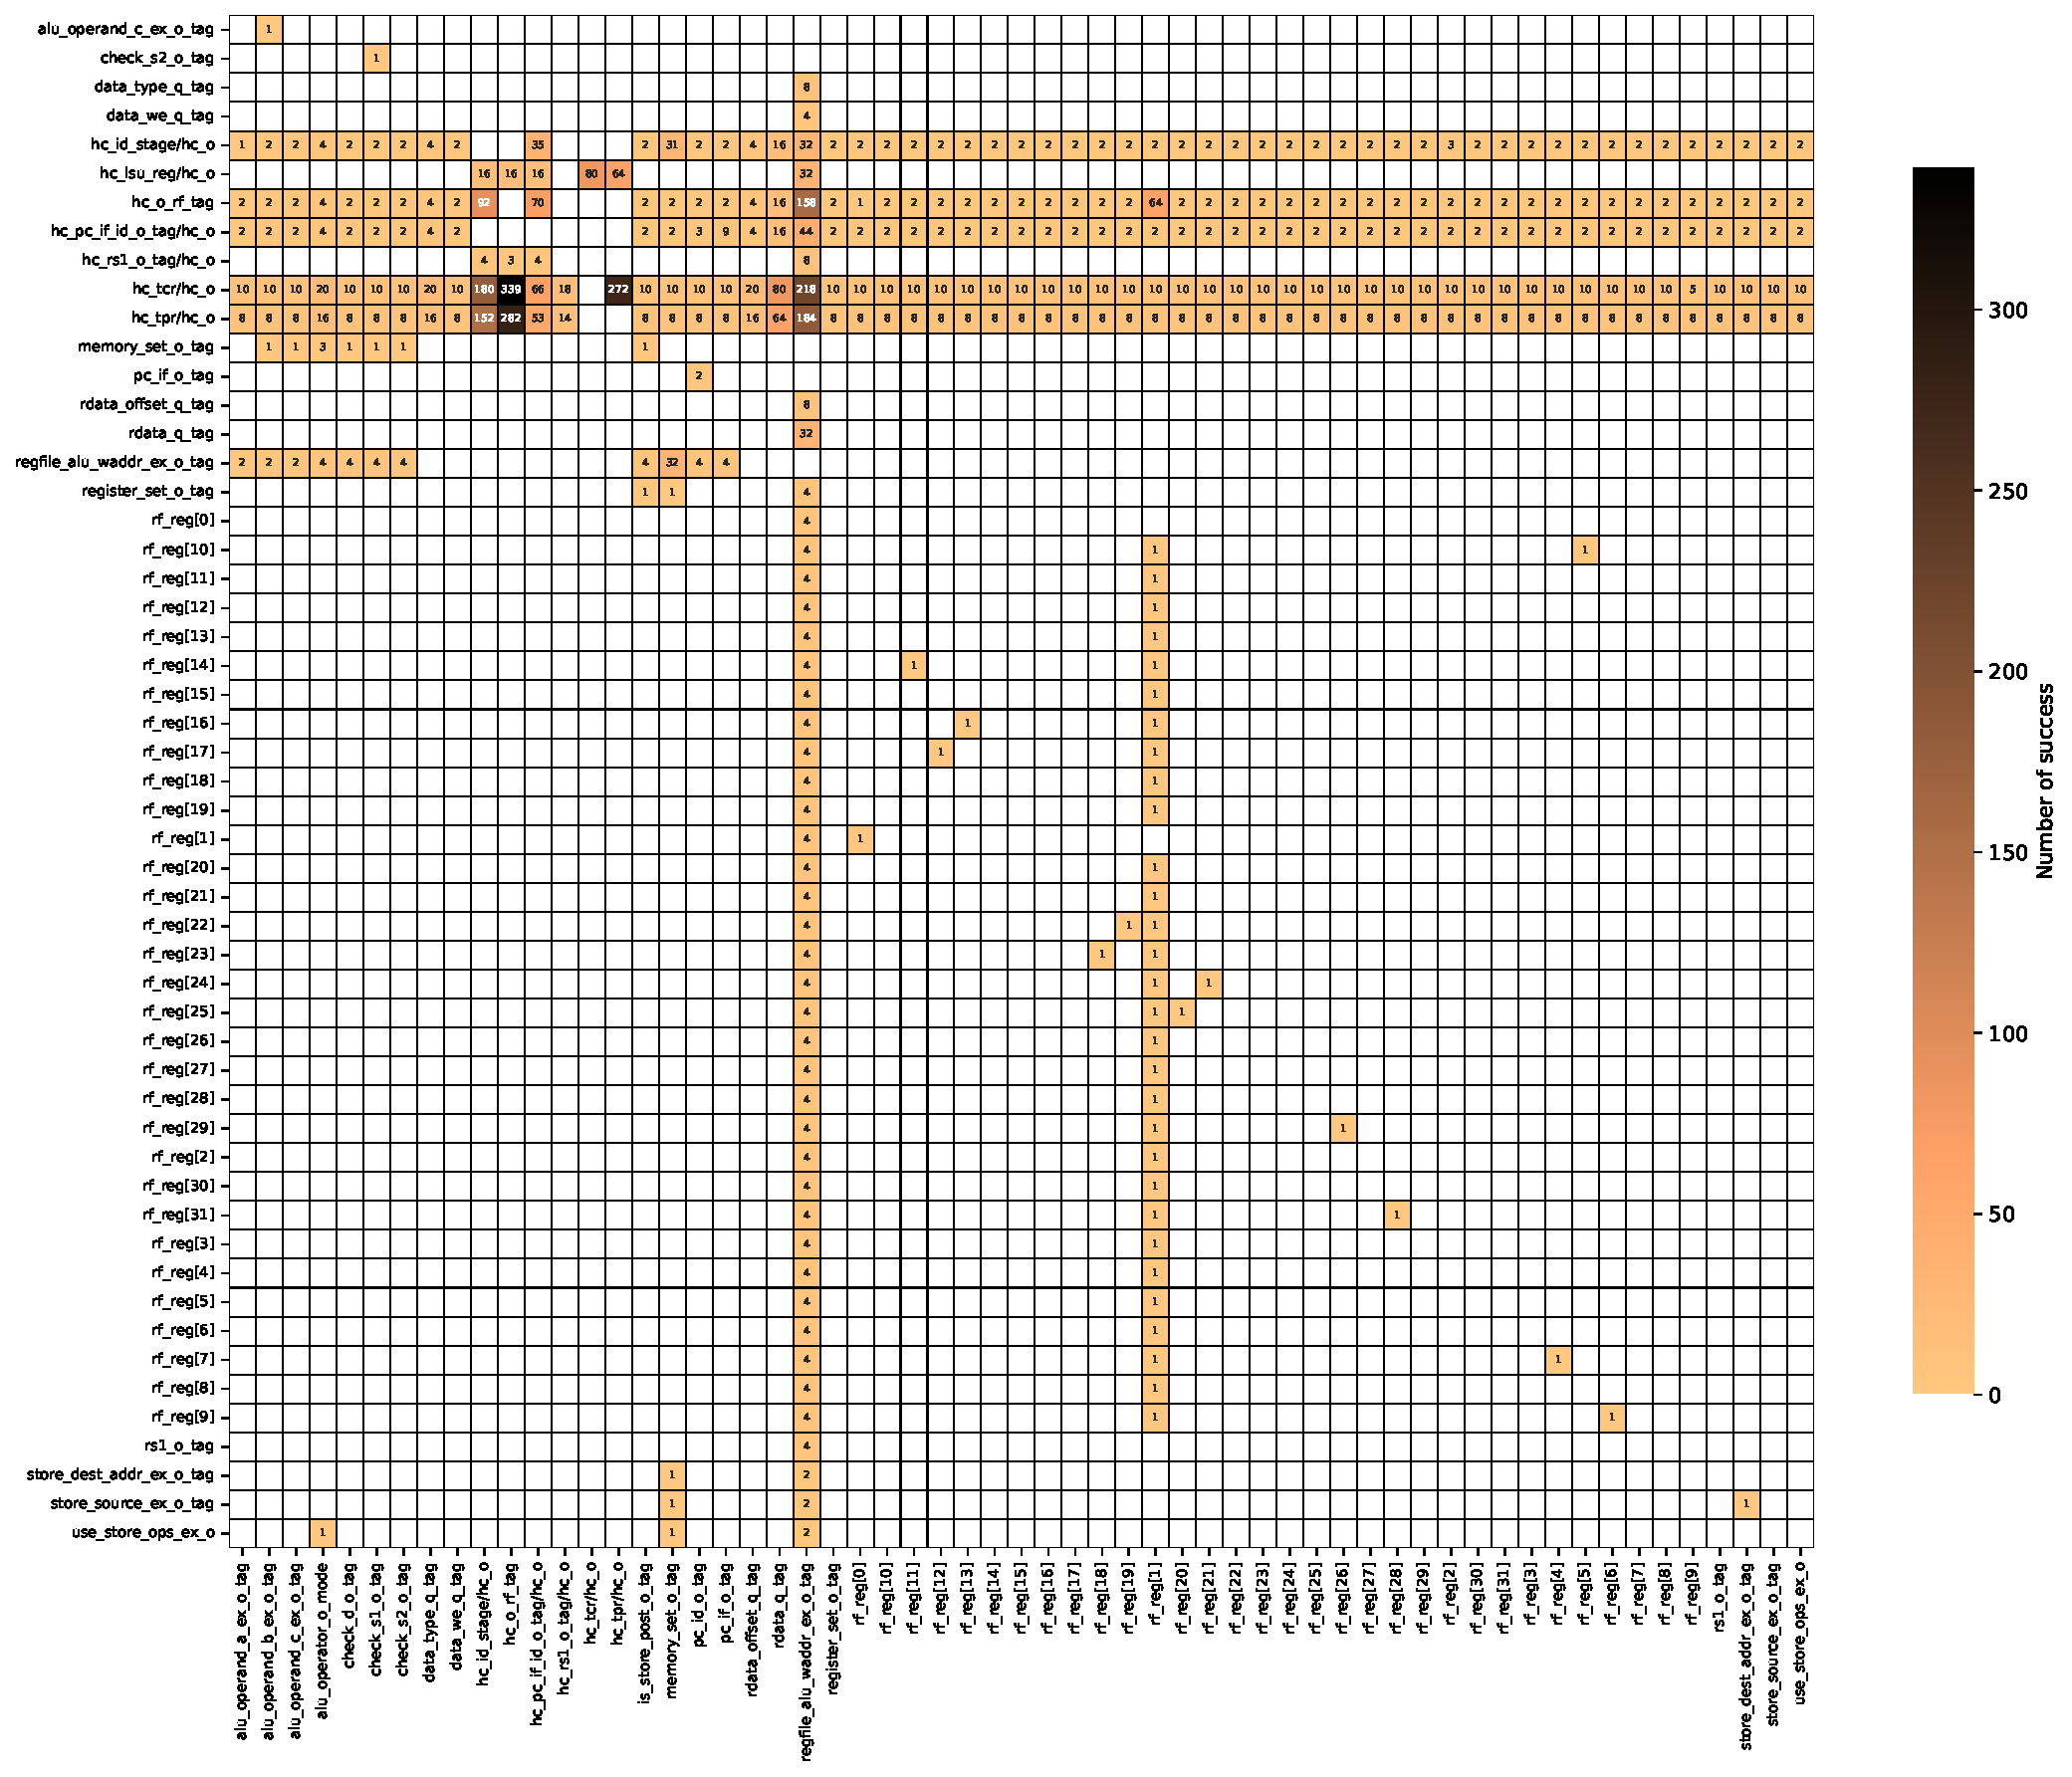
\includegraphics[width=\textwidth]{src/5_results/img/heatmap_buffer_overflow_hamming_2_multi_bitflip_reg_multi_2.pdf}
                \caption{Hamming Code 2 protected version: multi-bits faults in two registers at a given clock cycle $\rightarrow$ 4356 successes}
                \label{fig:heatmap_multibit_2}
            \end{figure}
        }
        \only<2>{
        \begin{figure}
            \centering
            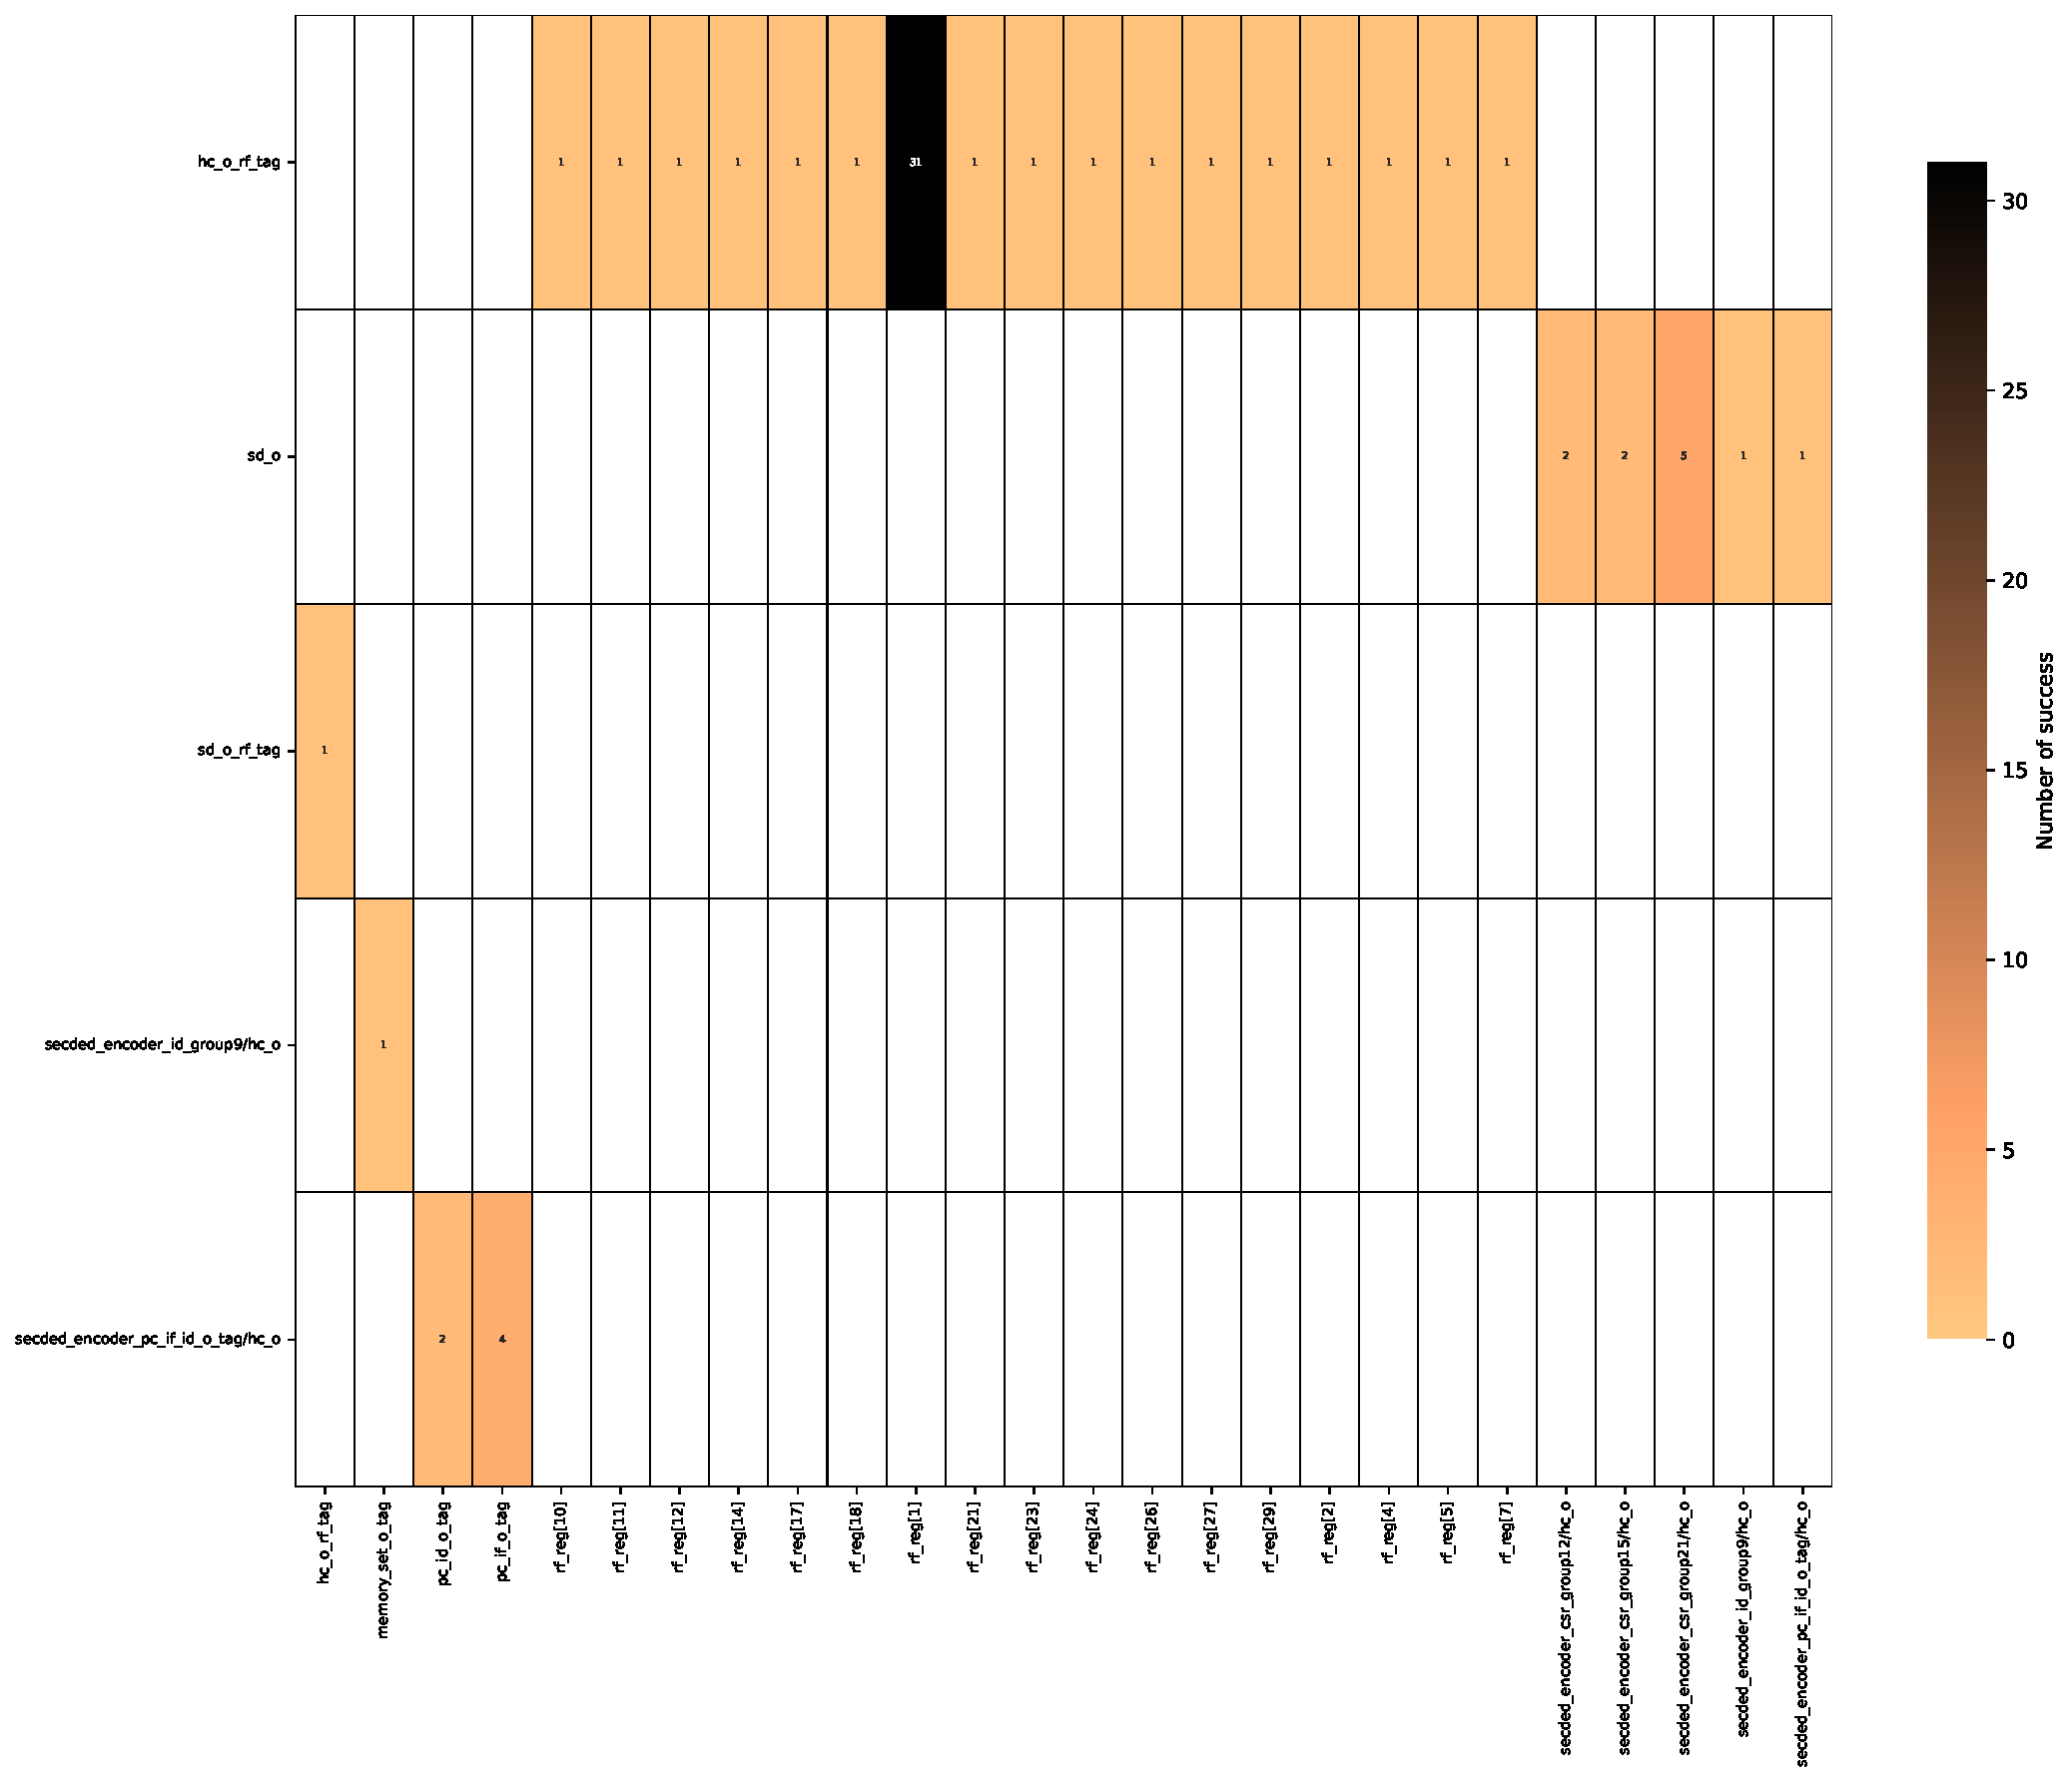
\includegraphics[width=\textwidth]{src/5_results/img/heatmap_buffer_overflow_secded_5_multi_bitflip_reg_multi_2.pdf}
            \caption{SECDED 5 protected version: multi-bits faults in two registers at a given clock cycle $\rightarrow$ 66 successes}
            \label{fig:heatmap_multibit_3}
        \end{figure}
        }
    \end{minipage}

    \note{HC2 augmente la surface d'attaque à cause du fait qu'il ne peut détecter et corriger 1 faute}
\end{frame}
%
% ---------------------------------------------------------------- %
\section{Conclusion and Perspectives}


%%%%%%%%%%%%%%%%%%%%%%%%%%%%%%%%%%%%%%%%%%%%%%%%%%%%%%%%%%%%%%%%%%%%%%%%%%%%
\subsection{Conclusion}
\begin{frame}{Conclusion}
    \begin{exampleblock}{}
        \centering
        How can we maintain maximum protection against software attacks in the presence of physical attacks?
    \end{exampleblock}
    
    \begin{columns}
        \begin{column}{.7\linewidth}
            \begin{block}{Presented:}
                \begin{itemize}
                    \setbeamertemplate{itemize items}[triangle]
                    \item<1> Vulnerability assessment of a DIFT mechanism against FIA
                        \only<1>{
                            \begin{itemize}
                                \item We have shown that the DIFT mechanism is vulnerable
                                \item Presented different fault models adapted from the state-of-the-art to defeat the DIFT and its protections
                            \end{itemize}
                        }
                    \item<2> Open-Source tool to help find vulnerabilities during the conceptual phase. It enables the concept of \textit{Security by Design}
                    \item<3> Proposition of 3 lightweight countermeasures with a low overhead of area and performances
                        \only<3>{
                            \begin{itemize}
                                \item countermeasures based on parity codes
                                \item area overhead smaller than 8\%
                                \item no impact on performances
                            \end{itemize}
                        }
                \end{itemize}
            \end{block}
        \end{column}
        \begin{column}{.3\linewidth}
            \begin{figure}
                \centering
                
\includegraphics[height=.25\textheight]{src/6_conclusion/img/conclusion.png}
            \end{figure}
        \end{column}
    \end{columns}
    
    \note{
        \textit{Vulnerability assessment:} taking into account different fault models up to very complex ones

        \textit{Countermeasures:} good efficiency, overhead is minimal compared to others countermeasures like BCH, spatial redundancy (duplication, triplication)
    }
\end{frame}

%%%%%%%%%%%%%%%%%%%%%%%%%%%%%%%%%%%%%%%%%%%%%%%%%%%%%%%%%%%%%%%%%%%%%%%%%%%%
\subsection{Perspectives}
\begin{frame}{Perspectives}
    \begin{block}{Short terms}
        \begin{itemize}
            \setbeamertemplate{itemize items}[triangle]
            \item<1> Propose more robust countermeasures to correct multiple faults
                \begin{itemize}
                    \item Evaluating of Reed-Solomon, BCH codes, or triplication
                    \item Evaluation of these countermeasures in terms of area and performances overhead compared to our actual proposed solutions
                \end{itemize}
            \item<2> Further development of FISSA
                \begin{itemize}
                    \item Better integration in the design workflow
                    \item More fault models
                    \item More configurability, for example, automatisation for finding targets
                    \item Adding a graphical user interface to provide better experience
                \end{itemize}
        \end{itemize}
    \end{block}
    
    \begin{figure}
        \centering
        
\includegraphics[height=.25\textheight]{src/6_conclusion/img/perspectives.jpg}
    \end{figure}
\end{frame}
%%%%%%%%%%%
\begin{frame}{Perspectives}
    \begin{block}{Long terms}
        \begin{itemize}
            \setbeamertemplate{itemize items}[triangle]
            \item Conduct real-world FIA
                \begin{itemize}
                    \item Evaluation against clock glitches (Chip Whisperer~\cite{chipwhisperer}) or EMFI (Chip Shouter~\cite{chipshouter}) for examples.
                \end{itemize}
            \item Extend the assessment of more complex DIFT
                \begin{itemize}
                    \item Evaluation of DIFT with more bits in the tag (e.g: Raksha~\cite{DKK-07-sigarch} : 4-bit tags)
                    \item Evaluation of our proposed protections for these DIFT and comparison with other protections
                \end{itemize}
        \end{itemize}
    \end{block}

    \begin{figure}
        \centering
        
\includegraphics[height=.25\textheight]{src/6_conclusion/img/perspectives.jpg}
    \end{figure}
\end{frame}
%%%%%%%%%%%%%%%%%%%%%%%%%%%%%%%%%%%%%%%%%%%%%%%%%%%%%%%%%%%%%%%%%%%%%%%%%%%%
%
% ---------------------------------------------------------------- %
\section*{Publications}

%%%%%%%%%%%%%%%%%%%%%%%%%%%%%%%%%%%%%%%%%%%%%%%%%%%%%%%%%%%%%%%%%%%%%%%%%%%%
\begin{frame}[allowframebreaks]{Publications}
    \begin{block}{International peer-reviewed conferences with proceedings}
        \begin{enumerate}
            \item {\footnotesize\textbf{William Pensec}, Vianney Lapôtre, and Guy Gogniat. 2023. Another Break in the Wall: Harnessing Fault Injection Attacks to Penetrate Software Fortresses. In Proceedings of the First International Workshop on Security and Privacy of Sensing Systems (SensorsS\&P), 2023. \textbf{Best paper award}~\cite{PLG-23-SensorsSP}}
            \item {\footnotesize\textbf{William Pensec}, Francesco Regazzoni, Vianney Lapôtre, and Guy Gogniat. Defending the Citadel: Fault Injection Attacks Against Dynamic Information Flow Tracking and Related Countermeasures. 2024 IEEE Computer Society Annual Symposium on VLSI (ISVLSI), 2024, pp. 180-185.~\cite{PRLG-24-isvlsi}}
            \item {\footnotesize\textbf{William Pensec}, Vianney Lapôtre, and Guy Gogniat. Scripting the Unpredictable: Automate Fault Injection in RTL Simulation for Vulnerability Assessment. 2024 27th Euromicro Conference on Digital System Design (DSD), 2024.~\cite{PLG-24-dsd}}
        \end{enumerate}
    \end{block}

    % \begin{block}{Conferences without proceedings}
    %     \begin{enumerate}
    %         \item {\footnotesize Vianney Lapôtre, \textbf{William Pensec} and Guy Gogniat, When in-core Dynamic Information Flow Tracking faces fault injection attacks, 19th International Workshops on Cryptographic architectures embedded in logic devices (CryptArchi), Cantabria, Spain, June 2023, \url{https://hal.science/hal-04381235}}
    %         \item {\footnotesize\textbf{William Pensec}, Vianney Lapôtre and Guy Gogniat, Unveiling the Invisible Threads: Dynamic Information Flow Tracking and the Intriguing World of Fault Injection Attacks, Journée thématique sur les Attaques par Injection de Fautes (JAIF), Gardanne, September 2023, \url{https://hal.science/hal-04727439}}
    %     \end{enumerate}
    % \end{block}

    \begin{block}{Source code}
        \begin{itemize}
            \item {\footnotesize \textbf{William Pensec}, FISSA: Fault Injection Simulation for Security Assessment, \url{https://github.com/WilliamPsc/FISSA}}
        \end{itemize}
    \end{block}

    \begin{block}{Popularising science event}
        \begin{itemize}
            \item {\footnotesize Participation in a science outreach event, “\textit{Ma thèse en 180 secondes}” (“My thesis in 180 seconds”), Rennes, March 2023, \url{https://youtu.be/m_whL8xGbMQ}}
        \end{itemize}
    \end{block}
\end{frame}
%%%%%%%%%%%%%%%%%%%%%%%%%%%%%%%%%%%%%%%%%%%%%%%%%%%%%%%%%%%%%%%%%%%%%%%%%%%%
\begin{frame}{}
    \backpage
\end{frame}
%%%%%%%%%%%%%%%%%%%%%%%%%%%%%%%%%%%%%%%%%%%%%%%%%%%%%%%%%%%%%%%%%%%%%%%%%%%%%%%%%%%%%%%%%%%%%%%%%%%%%%%%%%%%
%
% ---------------------------------------------------------------- %

\begin{frame}[noframenumbering]
    \vfill
    \centering
    \begin{beamercolorbox}[sep=8pt,center,shadow=true,rounded=true]{title}
        \usebeamerfont{section title} References
    \end{beamercolorbox}
    \vfill
\end{frame}

\begin{frame}[allowframebreaks, noframenumbering]{References}
    \printbibliography
\end{frame}
%
% ---------------------------------------------------------------- %
\section*{Backup}

%%%%%%%%%%%%%%%%%%%%%%%%%%%%%%%%%%%%%%%%%%%%%%%%%%%%%%%%%%%%%%%%%%%%%%%%%%%%
\begin{frame}[noframenumbering]{}
    \vfill
    \centering
    \begin{beamercolorbox}[sep=8pt,center,shadow=true,rounded=true]{title}
        \usebeamerfont{section title}\NoHyper\insertsection\par\endNoHyper
    \end{beamercolorbox}
    \vfill
\end{frame}
%%%%%%%%%%%%%%%%%%%%%%%%%%%%%%%%%%%%%%%%%%%%%%%%%%%%%%%%%%%%%%%%%%%%%%%%%%%%
\begin{frame}[noframenumbering]{Software threats: Dynamic Information Flow Tracking}
    \begin{minipage}[c]{0.4\textwidth}
        \begin{block}{}
            \begin{itemize}
                \setbeamertemplate{itemize items}[square]
                \justifying
                \item Static or \underline{\textbf{Dynamic}}
                \item Software, \underline{\textbf{Hardware}} or Hybrid
            \end{itemize}
        \end{block}
    \end{minipage}\hfill%
    \begin{minipage}[c]{0.55\textwidth}
        \begin{figure}
            \centering
            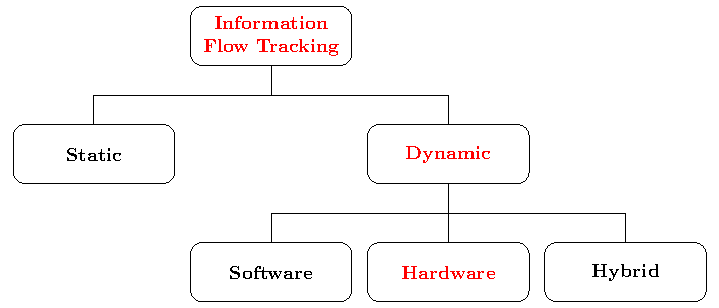
\includegraphics[width=\textwidth]{src/1_introduction/img/arborescence_ift.pdf}
            \caption{Taxonomy of IFTs}
            \label{fig:taxoDIFT}
        \end{figure}
    \end{minipage}
\end{frame}
%%%%%%%%%%%%%%%%%%%%%%%%%%%%%%%%%%%%%%%%%%%%%%%%%%%%%%%%%%%%%%%%%%%%%%%%%%%%
\begin{frame}[noframenumbering]{Tag Propagation Register}
    \begin{table}[!t]
        \centering
        \caption{Tag Propagation Register configuration}
        \label{tab:tpr}
        \resizebox{\linewidth}{!}{%
            \setlength{\tabcolsep}{2pt}
            \begin{tabular}{@{}lcccccccc@{}}
                \toprule
                          & Load/Store Enable & Load/Store Mode & Logical Mode & Comparison Mode & Shift Mode & Jump Mode & Branch Mode & Arith Mode \\ \cmidrule(lr){2-2}\cmidrule(lr){3-3}\cmidrule(lr){4-4}\cmidrule(lr){5-5}\cmidrule(lr){6-6}\cmidrule(lr){7-7}\cmidrule(lr){8-8}\cmidrule(lr){9-9}
                Bit index & 17 16 15          & 13 12           & 11 10        & 9 8             & 7 6        & 5 4       & 3 2         & 1 0        \\ \midrule
                Policy V1 & 0 0 1             & 1  0            & 1  0         & 0 0             & 1 0        & 1 0       & 0 0         & 1 0        \\
                Policy V2 & 1 1 1             & 1  0            & 1  0         & 1 0             & 1 0        & 1 0       & 1 0         & 1 0        \\ \bottomrule
            \end{tabular}
        }
    \end{table}

    \begin{itemize}
        \justifying
        \item A Mode field for each class of instructions which specifies how to propagate the tags of the input operands to the output operand tag.
              \begin{itemize}
                  \justifying
                  \item the output tag keeps its old value (00);
                  \item the output tag is set to one, if both the input tags are set to one (01);
                  \item the output tag is set to one, if at least one input tag is set to one (10);
                  \item the output tag is set to zero (11).
              \end{itemize}
        \item The three bits in the L/S enable field allow the policy to enable the source, source-address, and destination-address tags, respectively
    \end{itemize}
\end{frame}

\begin{frame}[noframenumbering]{Tag Check Register}
    \begin{table}[!t]
        \centering
        \caption{Tag Check Register configuration}
        \label{tab:tcr}
        \resizebox{\linewidth}{!}{%
            \setlength{\tabcolsep}{2pt}
            \begin{tabular}{@{}lcccccccc@{}}
                \toprule
                          & Execute Check & Load/Store Check & Logical Check & Comparison Check & Shift Check & Jump Check & Branch Check & Arith Check \\\cmidrule(lr){2-2}\cmidrule(lr){3-3}\cmidrule(lr){4-4}\cmidrule(lr){5-5}\cmidrule(lr){6-6}\cmidrule(lr){7-7}\cmidrule(lr){8-8}\cmidrule(lr){9-9}
                Bit index & 21            & 20 19 18 17      & 16 15 14      & 13 12 11         & 10 9 8      & 7 6 5      & 4 3          & 2 1 0       \\ \midrule
                Policy V1 & 1             & 1 0 1 0          & 0 0 0         & 0 0 0            & 0 0 0       & 0 0 0      & 0 0          & 0 0 0       \\
                Policy V2 & 0             & 0 0 0 0          & 0 0 0         & 0 0 0            & 0 0 0       & 0 0 0      & 0 0          & 0 1 1       \\ \bottomrule
            \end{tabular}
        }
    \end{table}

    \begin{itemize}
        \justifying
        \item The tag-check rules restrict the operations that may be performed on tagged data. If the check bit for an operand tag is set to one and the corresponding tag is equal to one, an exception is raised.
              \begin{itemize}
                  \justifying
                  \item For all the classes except Load/Store, there are three tags to consider: first input, second input, and output tags
                  \item For the Load/Store class there are four tags to take into account: source-address, source, destination-address, and destination tags
                  \item the additional Execute Check field is associated with the program counter and specifies whether to raise a security exception when the program-counter tag is set to one
              \end{itemize}
    \end{itemize}
\end{frame}
%%%%%%%%%%%%%%%%%%%%%%%%%%%%%%%%%%%%%%%%%%%%%%%%%%%%%%%%%%%%%%%%%%%%%%%%%%%%
\begin{frame}[noframenumbering]{Case 1: Buffer Overflow}
    \begin{table}[H]
        \scriptsize
        \centering
        \caption{Logical fault injection simulation campaigns results for exhaustive multi-bits faults in one register at a given clock cycle}
        \label{tab:chap6_results_multi_bitflip_reg_bo}
        \setlength{\tabcolsep}{3pt}
        \begin{tabular}{@{}ccccccccccc@{}}
            \toprule
                                                               &                & Crash & Silent & Delay & Detection & \tableTwoLines{Detection \&}{Correction} & \tableTwoLines{Double Error}{Detection} & Success                                       & Total       & \tableTwoLines{Execution}{time (h:min)} \\\midrule
            \multirow{12}{*}{\tableTwoLines{Buffer}{Overflow}} & No protection  & 0     & 927    & 6     & --        & --                                       & --                                      & 3 {\tiny (0.32\%)}                            & 936         & 00:08                           \\
                                                               & Simple parity  & 0     & 498    & 0     & 498       & --                                       & --                                      & 0                                             & 996         & 00:14                           \\
                                                               & Hamming 1 & 0     & 0      & 20    & --        & 1962                                     & --                                      & 10 {\tiny (0.50\%)}                           & 1992        & 00:28                           \\
                                                               & Hamming 2 & 0     & 0      & 12    & --        & 2038                                     & --                                      & 14 {\tiny (0.68\%)}                           & 2064        & 00:32                           \\
                                                               & Hamming 3 & 0     & 0      & 12    & --        & 2352                                     & --                                      & 12 {\tiny (0.51\%)}                           & 2376        & 00:28                           \\
                                                               & Hamming 4 & 0     & 0      & 12    & --        & 2712                                     & --                                      & 12 {\tiny (0.44\%)}                           & 2736        & 00:35                           \\
                                                               & Hamming 5 & 0     & 0      & 12    & --        & 2976                                     & --                                      & 12 {\tiny (0.40\%)}                           & 3000        & 00:45                           \\
                                                               & SECDED 1       & 0     & 0      & 8     & --        & 1393                                     & 648                                     & 3 {\tiny (0.15\%)}                            & 2052        & 00:30                           \\
                                                               & SECDED 2       & 0     & 0      & 5     & --        & 1475                                     & 666                                     & 2 {\tiny (0.09\%)}                            & 2148        & 00:30                           \\
                                                               & SECDED 3       & 0     & 0      & 4     & --        & 1932                                     & 726                                     & 2 {\tiny (0.08\%)}                            & 2664        & 00:40                           \\
                                                               & SECDED 4       & 0     & 0      & 0     & --        & 2370                                     & 822                                     & 0                                             & 3192        & 00:45                           \\
                                                               & SECDED 5       & 0     & 0      & 0     & --        & 2670                                     & 798                                     & 0                                             & 3468        & 00:55                           \\
            \bottomrule
        \end{tabular}
    \end{table}
\end{frame}
%%%%%%%%%%%%%%%%%%%%%%%%%%%%%%%%%%%%%%%%%%%%%%%%%%%%%%%%%%%%%%%%%%%%%%%%%%%%
\begin{frame}[fragile,noframenumbering]{Case 2: WU-FTPd}
    \begin{itemize}
        \justifying
        \item The vulnerability is the use of an unchecked user input as the format string parameter in functions that perform formatting, e.g. printf()
        \item An attacker can use the format tokens, to write into arbitrary locations of memory, e.g. the return address of the function.
    \end{itemize}

    \centering
    \begin{minipage}[c]{\textwidth}
        \begin{lstlisting}[language=C,label=code:printfNFormat]
void echo(){
    int a;
    register int i asm("x8");
    a = i;
    printf("%224u%n%35u%n%253u%n%n", 1, (int*) (a-4), 1, (int*) (a-3), 1, (int*) (a-2), (int*) (a-1));
}\end{lstlisting}
    \end{minipage}
\end{frame}

\begin{frame}[noframenumbering]{Case 2: WU-FTPd}
    \begin{figure}
        \centering
        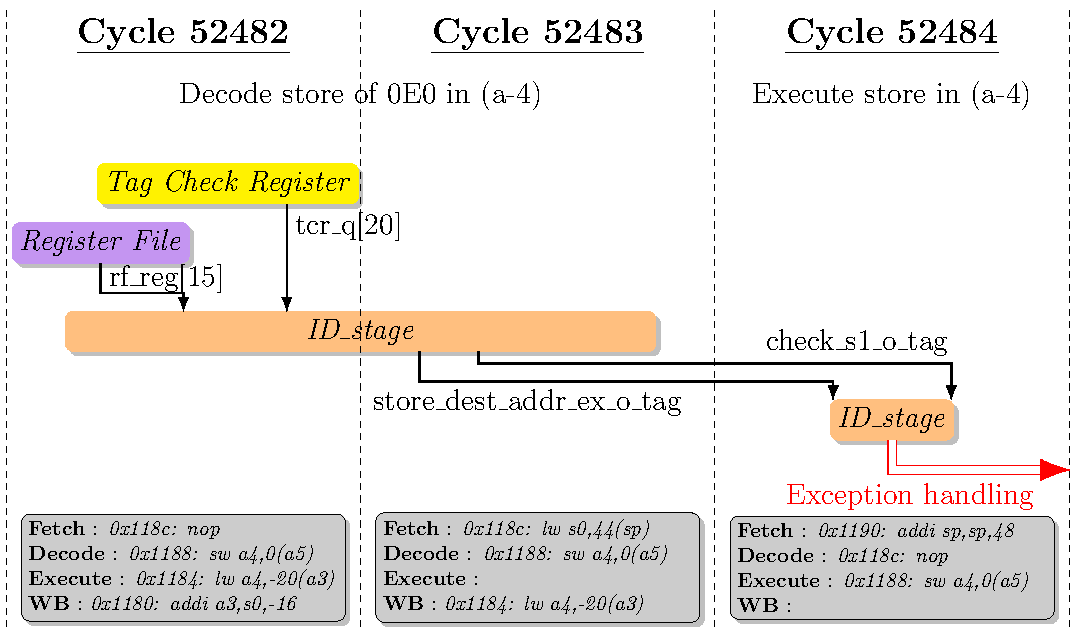
\includegraphics[height=.85\textheight]{src/2_vuln_assessment/img/wuftpd/ftpd_short.pdf}
        \caption{Temporal analysis of the tags propagation in a \textit{format string} attack}
        \label{fig:analyseTempoFormatString}
    \end{figure}
\end{frame}

\begin{frame}[noframenumbering]{Case 2: WU-FTPd}
    \begin{figure}
        \centering
        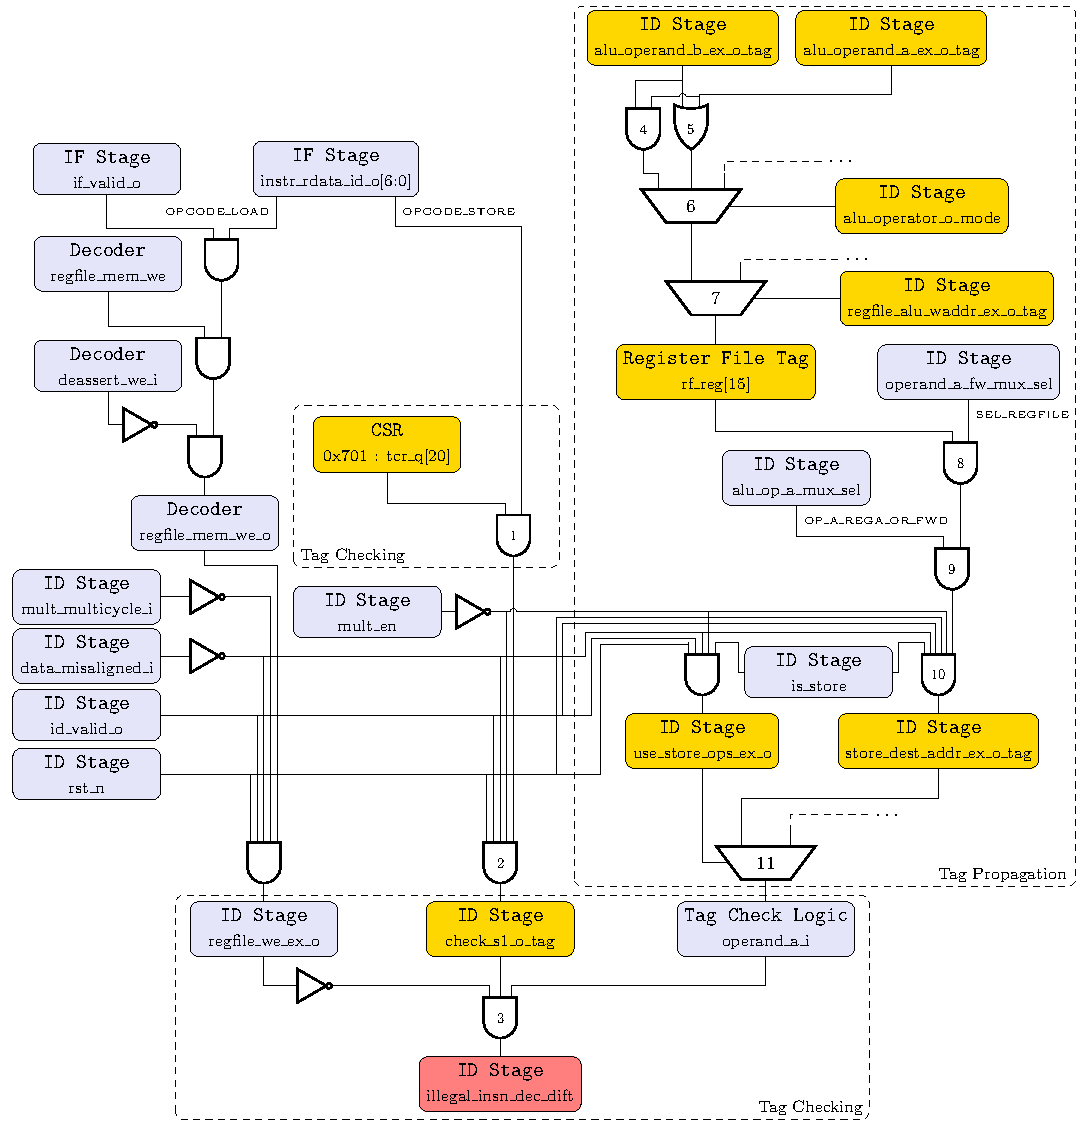
\includegraphics[height=.85\textheight]{src/2_vuln_assessment/img/wuftpd/arborescence_wuftpd.pdf}
        \caption{Logical analysis of the tags propagation in a \textit{format string} attack}
        \label{fig:analyseLogiqueFormatString}
    \end{figure}
\end{frame}

\begin{frame}[noframenumbering]{Case 2: WU-FTPd}
    \begin{table}[H]
        \scriptsize
        \centering
        \caption{Logical fault injection simulation campaigns results for single bit-flip in two registers at a given clock cycle}
        \label{tab:chap6_results_single_bitflip_spatial_fs}
        \setlength{\tabcolsep}{2pt}
        \begin{tabular}{@{}ccccccccccc@{}}
            \toprule
                                                             &               & Crash & Silent      & Delay      & Detection   & \tableTwoLines{Detection \&}{Correction} & \tableTwoLines{Double Error}{Detection} & Success                     & Total        & \tableTwoLines{Execution}{time (h:min)} \\\midrule
            \multirow{12}{*}{\tableTwoLines{Format}{String}} & No protection & 0     & \num{55589} & \num{5035} & --          & --                                       & --                                      & \num{3384} {\tiny (5.29\%)} & \num{64008}  & 163:09                                  \\
                                                             & Simple parity & 0     & \num{13361} & 450        & \num{54590} & --                                       & --                                      & 767  {\tiny (1.11\%)}       & \num{69168 } & 114:06                                  \\
                                                             & Hamming 1     & 0     & 0           & 1709       & --          & \num{89010 }                             & --                                      & 1089 {\tiny (1.19\%)}       & \num{91808 } & 179:38                                  \\
                                                             & Hamming 2     & 0     & 0           & 982        & --          & \num{96182 }                             & --                                      & 804  {\tiny (0.82\%)}       & \num{97968 } & 136:40                                  \\
                                                             & Hamming 3     & 0     & 0           & 659        & --          & \num{143883}                             & --                                      & 618  {\tiny (0.43\%)}       & \num{145160} & 261:40                                  \\
                                                             & Hamming 4     & 0     & 0           & 379        & --          & \num{206423}                             & --                                      & 222  {\tiny (0.11\%)}       & \num{207024} & 368:10                                  \\
                                                             & Hamming 5     & 0     & 0           & 391        & --          & \num{230758}                             & --                                      & 211  {\tiny (0.09\%)}       & \num{231360} & 445:58                                  \\
                                                             & SECDED 1      & 0     & 0           & 0          & --          & \num{82480 }                             & \num{15488}                             & 0                           & \num{97968 } & 233:28                                  \\
                                                             & SECDED 2      & 0     & 0           & 0          & --          & \num{92472 }                             & \num{14456}                             & 0                           & \num{106928} & 185:35                                  \\
                                                             & SECDED 3      & 0     & 0           & 0          & --          & \num{171168}                             & \num{12872}                             & 0                           & \num{184040} & 317:20                                  \\
                                                             & SECDED 4      & 0     & 0           & 0          & --          & \num{272080}                             & \num{9880 }                             & 0                           & \num{281960} & 462:58                                  \\
                                                             & SECDED 5      & 0     & \num{16128} & 0          & --          & \num{286296}                             & \num{10056}                             & 0                           & \num{312480} & 558:16                                  \\
            \bottomrule
        \end{tabular}
    \end{table}
\end{frame}

\begin{frame}[noframenumbering]{Case 2: WU-FTPd}
    \begin{table}[H]
        \scriptsize
        \centering
        \caption{Logical fault injection simulation campaigns results for exhaustive multi-bits faults in one register at a given clock cycle}
        \label{tab:chap6_results_multi_bitflip_reg_fs}
        \setlength{\tabcolsep}{3pt}
        \begin{tabular}{@{}ccccccccccc@{}}
            \toprule
                                                               &                & Crash & Silent & Delay & Detection & \tableTwoLines{Detection \&}{Correction} & \tableTwoLines{Double Error}{Detection} & Success                                       & Total       & \tableTwoLines{Execution}{time (h:min)} \\\midrule
            \multirow{12}{*}{\tableTwoLines{Format}{String}}   & No protection  & 0     & 1202   & 32    & --        & --                                       & --                                      & 14 {\tiny (1.12\%)}                           & 1248        & 01:24                           \\
                                                               & Simple parity  & 0     & 661    & 0     & 665       & --                                       & --                                      & 2  {\tiny (0.15\%)}                           & 1328        & 02:12                           \\
                                                               & Hamming 1 & 0     & 0      & 62    & --        & 2565                                     & --                                      & 29 {\tiny (1.09\%)}                           & 2656        & 04:24                           \\
                                                               & Hamming 2 & 0     & 0      & 53    & --        & 2666                                     & --                                      & 33 {\tiny (1.20\%)}                           & 2752        & 03:36                           \\
                                                               & Hamming 3 & 0     & 0      & 47    & --        & 3090                                     & --                                      & 31 {\tiny (0.98\%)}                           & 3168        & 03:55                           \\
                                                               & Hamming 4 & 0     & 0      & 47    & --        & 3570                                     & --                                      & 31 {\tiny (0.85\%)}                           & 3648        & 04:25                           \\
                                                               & Hamming 5 & 0     & 0      & 41    & --        & 3930                                     & --                                      & 29 {\tiny (0.73\%)}                           & 4000        & 05:18                           \\
                                                               & SECDED 1       & 0     & 0      & 22    & --        & 1832                                     & 864                                     & 18 {\tiny (0.66\%)}                           & 2736        & 03:30                           \\
                                                               & SECDED 2       & 0     & 0      & 14    & --        & 1938                                     & 894                                     & 18 {\tiny (0.63\%)}                           & 2864        & 03:48                           \\
                                                               & SECDED 3       & 0     & 0      & 10    & --        & 2560                                     & 968                                     & 14 {\tiny (0.39\%)}                           & 3552        & 04:42                           \\
                                                               & SECDED 4       & 0     & 0      & 5     & --        & 3146                                     & 1096                                    & 9  {\tiny (0.21\%)}                           & 4256        & 05:42                           \\
                                                               & SECDED 5       & 0     & 0      & 4     & --        & 3554                                     & 1064                                    & 2  {\tiny (0.04\%)}                           & 4624        & 06:30                           \\
            \bottomrule
        \end{tabular}
    \end{table}
\end{frame}

\begin{frame}[noframenumbering]{Case 2: WU-FTPd}
    \begin{table}[H]
        \scriptsize
        \centering
        \caption{Logical fault injection simulation campaigns results for exhaustive multi-bits faults in two registers at a given clock cycle}
        \label{tab:chap6_results_multi_bitflip_reg_multi_fs}
        \setlength{\tabcolsep}{1pt}
        \begin{tabular}{@{}ccccccccccc@{}}
            \toprule
                                                             &               & Crash & Silent      & Delay       & Detection   & \tableTwoLines{Detection \&}{Correction} & \tableTwoLines{Double Error}{Detection} & Success                      & Total          & \tableTwoLines{Execution}{time (h:min)} \\\midrule
            \multirow{12}{*}{\tableTwoLines{Format}{String}} & No protection & 0     & \num{84419} & 4836        & --          & --                                       & --                                      & 2009 {\tiny (2.20\%)}        & \num{91264 }   & 104:15                                  \\
                                                             & Simple parity & 0     & \num{32275} & 147         & \num{71198} & --                                       & --                                      & 444 {\tiny (0.43\%)}         & \num{104064}   & 138:40                                  \\
                                                             & Hamming 1     & 0     & 0           & \num{20050} & --          & \num{375836}                             & --                                      & 9234 {\tiny (2.28\%)}        & \num{405120}   & 902:08                                  \\
                                                             & Hamming 2     & 0     & 0           & \num{17597} & --          & \num{408894}                             & --                                      & \num{10757} {\tiny (2.46\%)} & \num{437248}   & 774:40                                  \\
                                                             & Hamming 3     & 0     & 0           & \num{17926} & --          & \num{564154}                             & --                                      & \num{11456} {\tiny (1.93\%)} & \num{593536}   & 1021:50                                 \\
                                                             & Hamming 4     & 0     & 0           & \num{20986} & --          & \num{767604}                             & --                                      & \num{13714} {\tiny (1.71\%)} & \num{802304}   & 1418:24                                 \\
                                                             & Hamming 5     & 0     & 0           & \num{20547} & --          & \num{934077}                             & --                                      & \num{14336} {\tiny (1.48\%)} & \num{968960}   & 1690:05                                 \\
                                                             & SECDED 1      & 0     & 0           & 5408        & --          & \num{194766}                             & \num{227655}                            & 4171 {\tiny (0.97\%)}        & \num{432000}   & 740:21                                  \\
                                                             & SECDED 2      & 0     & 0           & 3611        & --          & \num{220568}                             & \num{247704}                            & 4565 {\tiny (0.96\%)}        & \num{476448}   & 836:41                                  \\
                                                             & SECDED 3      & 0     & 0           & 3088        & --          & \num{395487}                             & \num{351553}                            & 4304 {\tiny (0.57\%)}        & \num{754432}   & 1305:36                                 \\
                                                             & SECDED 4      & 0     & 0           & 1939        & --          & \num{604649}                             & \num{491945}                            & 3515 {\tiny (0.32\%)}        & \num{1102048}  & 1915:20                                 \\
                                                             & SECDED 5      & 0     & 0           & 1938        & --          & \num{766527}                             & \num{535209}                            & 998 {\tiny (0.08\%)}         & \num{1304672}  & 2287:38                                 \\
            \bottomrule
        \end{tabular}
    \end{table}
\end{frame}
%%%%%%%%%%%%%%%%%%%%%%%%%%%%%%%%%%%%%%%%%%%%%%%%%%%%%%%%%%%%%%%%%%%%%%%%%%%%%%%%%%%%%%%%%%%%%%%%%%%%%%%%%%%%
\begin{frame}[fragile,noframenumbering]{Case 3: Compare/Compute}
    \begin{itemize}
        \justifying
        \item No software vulnerability
        \item Used to cover the DIFT surface
    \end{itemize}

    \centering
    \begin{minipage}[c]{\textwidth}
        \begin{lstlisting}[language=C,label=code:compareCompute]
int main(){
    int a, b = 5, c;
    register int reg asm("x9");
    a = reg;
    asm volatile("csrw 0x700, tprValue");
    asm volatile("csrw 0x701, tcrValue");
    asm volatile("p.spsw x0, 0(\%0);" :: "r" (&a));
    c = (a > b) ? (a-b) : (a+b);
        //42c:   ble a4,a5,448
        //430:   addi a5,s0,-16
        //434:   lw a4,-12(a5)
        //438:   addi a3,s0,-16
        //43c:   lw a5,-4(a3)
        //440:   sub a5,a4,a5
        //444:   j 45c
        //448:   addi a5,s0,-16
        //44c:   lw a4,-12(a5)
        //450:   addi a3,s0,-16
        //454:   lw a5,-4(a3)
        //458:   add a5,a4,a5
        //45c:   sw a5,-24(s0)
    return EXIT_SUCCESS;
}\end{lstlisting}
    \end{minipage}
\end{frame}

\begin{frame}[noframenumbering]{Case 3: Compare/Compute}
    \begin{figure}
        \centering
        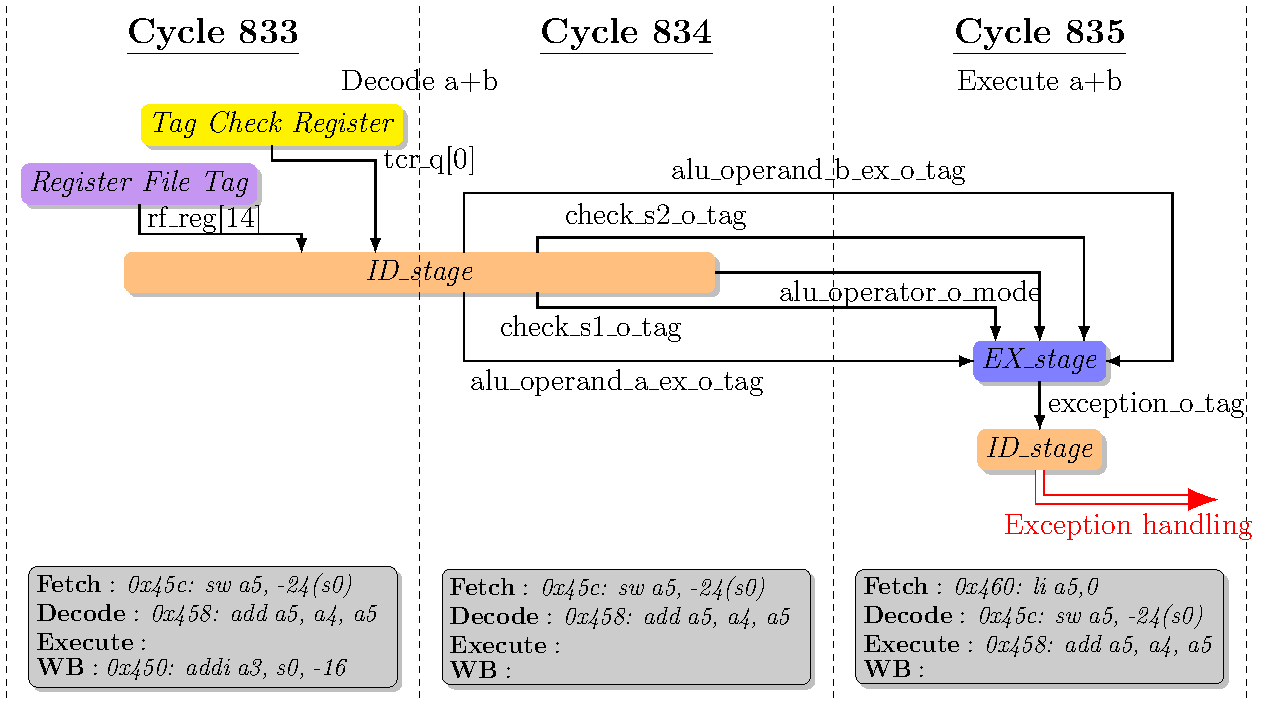
\includegraphics[height=.85\textheight]{src/2_vuln_assessment/img/comp_compu/attaquePropag_v3_short.pdf}
        \caption{Temporal analysis of the tags propagation in a \textit{format string} attack}
        \label{fig:analyseTempoCompCompute}
    \end{figure}
\end{frame}

\begin{frame}[noframenumbering]{Case 3: Compare/Compute}
    \begin{figure}
        \centering
        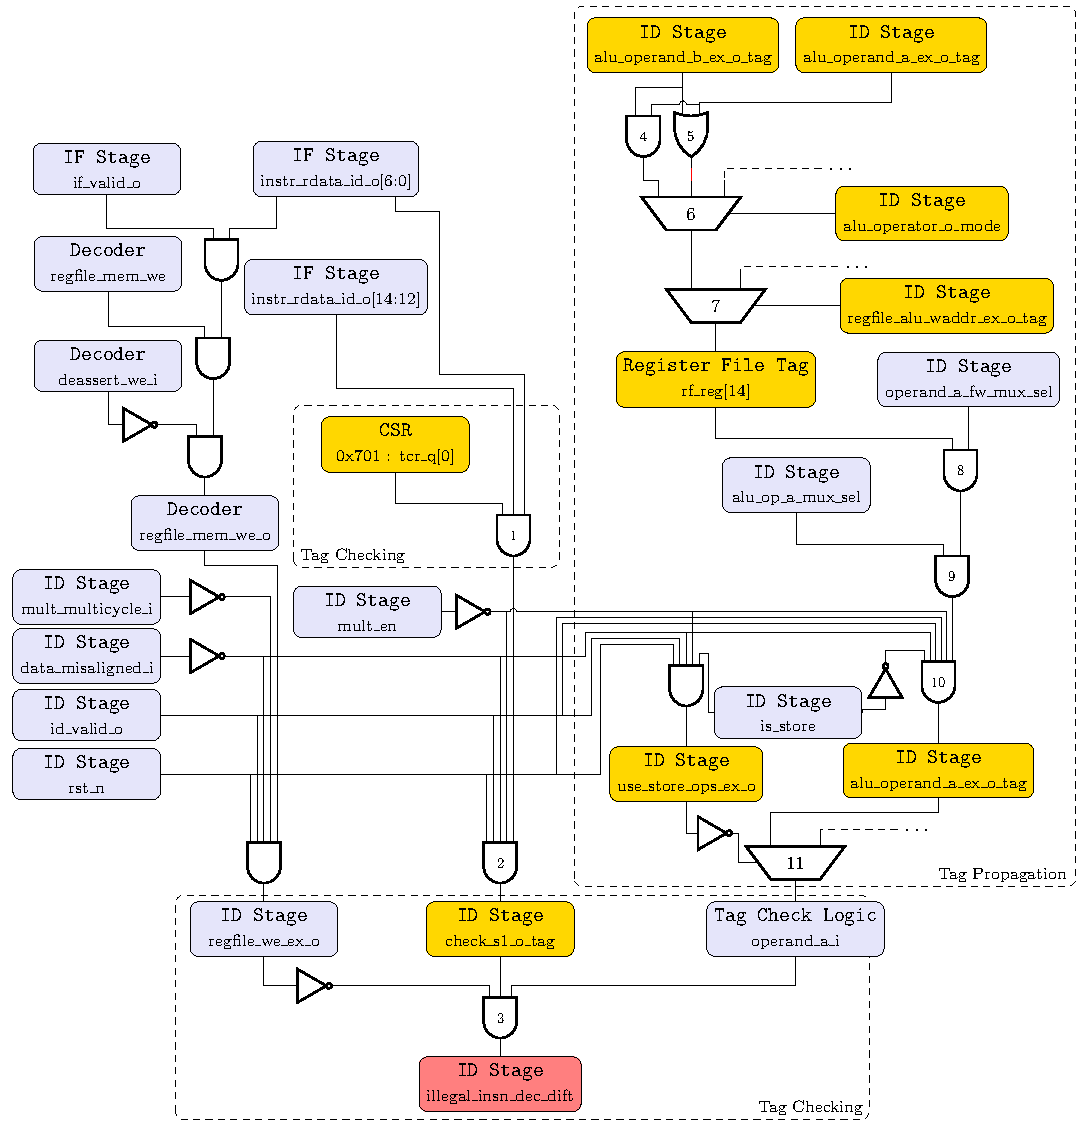
\includegraphics[height=.85\textheight]{src/2_vuln_assessment/img/comp_compu/arborescence_propagation.pdf}
        \caption{Logical analysis of the tags propagation in a \textit{format string} attack}
        \label{fig:analyseLogiqueCompCompute}
    \end{figure}
\end{frame}

\begin{frame}[noframenumbering]{Case 3: Compare/Compute}
    \begin{table}[H]
        \scriptsize
        \centering
        \caption{Logical fault injection simulation campaigns results for single bit-flip in two registers at a given clock cycle}
        \label{tab:chap6_results_single_bitflip_spatial_cc}
        \setlength{\tabcolsep}{2pt}
        \begin{tabular}{@{}ccccccccccc@{}}
            \toprule
                                                               &               & Crash & Silent      & Delay & Detection   & \tableTwoLines{Detection \&}{Correction} & \tableTwoLines{Double Error}{Detection} & Success                                              & Total         & \tableTwoLines{Execution}{time (h:min)} \\\midrule
            \multirow{12}{*}{\tableTwoLines{Compare}{Compute}} & No protection & 0     & \num{29906} & 919   & --          & --                                       & --                                      & \num{1179} {\tiny (3.68\%)}                          & \num{32004}   & 05:24                                   \\
                                                               & Simple parity & 0     & \num{6697}  & 202   & \num{27678} & --                                       & --                                      & 7   {\tiny (0.02\%)}                                 & \num{34584 }  & 04:48                                   \\
                                                               & Hamming 1     & 0     & 0           & 450   & --          & \num{45192  }                            & --                                      & 262 {\tiny (0.57\%)}                                 & \num{45904 }  & 09:21                                   \\
                                                               & Hamming 2     & 0     & 0           & 440   & --          & \num{48419  }                            & --                                      & 125 {\tiny (0.26\%)}                                 & \num{48984 }  & 08:47                                   \\
                                                               & Hamming 3     & 0     & 0           & 315   & --          & \num{72140  }                            & --                                      & 125 {\tiny (0.17\%)}                                 & \num{72580 }  & 13:53                                   \\
                                                               & Hamming 4     & 0     & 0           & 97    & --          & \num{103345 }                            & --                                      & 70  {\tiny (0.07\%)}                                 & \num{103512}  & 22:23                                   \\
                                                               & Hamming 5     & 0     & 0           & 96    & --          & \num{115511 }                            & --                                      & 73  {\tiny (0.06\%)}                                 & \num{115680}  & 23:48                                   \\
                                                               & SECDED 1      & 0     & 0           & 0     & --          & \num{37740  }                            & \num{11244}                             & 0                                                    & \num{48984 }  & 17:00                                   \\
                                                               & SECDED 2      & 0     & 0           & 0     & --          & \num{46236  }                            & \num{7228}                              & 0                                                    & \num{53464 }  & 10:12                                   \\
                                                               & SECDED 3      & 0     & 0           & 0     & --          & \num{85584  }                            & \num{6436}                              & 0                                                    & \num{92020 }  & 18:25                                   \\
                                                               & SECDED 4      & 0     & 0           & 0     & --          & \num{136040 }                            & \num{4940}                              & 0                                                    & \num{140980}  & 28:37                                   \\
                                                               & SECDED 5      & 0     & 0           & 0     & --          & \num{151212 }                            & \num{5028}                              & 0                                                    & \num{156240}  & 32:52                                   \\
            \bottomrule
        \end{tabular}
    \end{table}
\end{frame}

\begin{frame}[noframenumbering]{Case 3: Compare/Compute}
    \begin{table}[H]
        \scriptsize
        \centering
        \caption{Logical fault injection simulation campaigns results for exhaustive multi-bits faults in one register at a given clock cycle}
        \label{tab:chap6_results_multi_bitflip_reg_cc}
        \setlength{\tabcolsep}{3pt}
        \begin{tabular}{@{}ccccccccccc@{}}
            \toprule
                                                               &                & Crash & Silent & Delay & Detection & \tableTwoLines{Detection \&}{Correction} & \tableTwoLines{Double Error}{Detection} & Success                                       & Total       & \tableTwoLines{Execution}{time (h:min)} \\\midrule
            \multirow{12}{*}{\tableTwoLines{Compare}{Compute}} & No protection  & 0     & 616    & 2     & --        & --                                       & --                                      & 6  {\tiny (0.96\%)}                           & 624         & 00:04                           \\
                                                               & Simple parity  & 0     & 330    & 0     & 334       & --                                       & --                                      & 0                                             & 664         & 00:04                           \\
                                                               & Hamming 1 & 0     & 0      & 9     & --        & 1311                                     & --                                      & 8 {\tiny (0.60\%)}                            & 1328        & 00:09                           \\
                                                               & Hamming 2 & 0     & 0      & 15    & --        & 1356                                     & --                                      & 5 {\tiny (0.36\%)}                            & 1376        & 00:09                           \\
                                                               & Hamming 3 & 0     & 0      & 12    & --        & 1567                                     & --                                      & 5 {\tiny (0.32\%)}                            & 1584        & 00:11                           \\
                                                               & Hamming 4 & 0     & 0      & 12    & --        & 1807                                     & --                                      & 5 {\tiny (0.27\%)}                            & 1824        & 00:13                           \\
                                                               & Hamming 5 & 0     & 0      & 12    & --        & 1983                                     & --                                      & 5 {\tiny (0.25\%)}                            & 2000        & 00:14                           \\
                                                               & SECDED 1       & 0     & 0      & 2     & --        & 888                                      & 476                                     & 2 {\tiny (0.15\%)}                            & 1368        & 00:09                           \\
                                                               & SECDED 2       & 0     & 0      & 6     & --        & 977                                      & 449                                     & 0                                             & 1432        & 00:10                           \\
                                                               & SECDED 3       & 0     & 0      & 2     & --        & 1290                                     & 484                                     & 0                                             & 1776        & 00:12                           \\
                                                               & SECDED 4       & 0     & 0      & 0     & --        & 1580                                     & 548                                     & 0                                             & 2128        & 00:15                           \\
                                                               & SECDED 5       & 0     & 0      & 0     & --        & 1780                                     & 532                                     & 0                                             & 2312        & 00:16                           \\
            \bottomrule
        \end{tabular}
    \end{table}
\end{frame}

\begin{frame}[noframenumbering]{Case 3: Compare/Compute}
    \begin{table}[H]
        \scriptsize
        \centering
        \caption{Logical fault injection simulation campaigns results for exhaustive multi-bits faults in two registers at a given clock cycle}
        \label{tab:chap6_results_multi_bitflip_reg_multi_cc}
        \setlength{\tabcolsep}{1pt}
        \begin{tabular}{@{}ccccccccccc@{}}
            \toprule
                                                               &               & Crash & Silent      & Delay & Detection   & \tableTwoLines{Detection \&}{Correction} & \tableTwoLines{Double Error}{Detection} & Success               & Total        & \tableTwoLines{Execution}{time (h:min)} \\\midrule
            \multirow{12}{*}{\tableTwoLines{Compare}{Compute}} & No protection & 0     & \num{44444} & 323   & --          & --                                       & --                                      & 865 {\tiny (1.90\%)}  & \num{45632 } & 05:36                                   \\
                                                               & Simple parity & 0     & \num{16033} & 53    & \num{35943} & --                                       & --                                      & 3 {\tiny (0.01\%)}    & \num{52032 } & 08:05                                   \\
                                                               & Hamming 1     & 0     & 0           & 2912  & --          & \num{196958}                             & --                                      & 2690 {\tiny (1.33\%)} & \num{202560} & 34:17                                   \\
                                                               & Hamming 2     & 0     & 0           & 4677  & --          & \num{211969}                             & --                                      & 1978 {\tiny (0.90\%)} & \num{218624} & 37:24                                   \\
                                                               & Hamming 3     & 0     & 0           & 4377  & --          & \num{290302}                             & --                                      & 2089 {\tiny (0.70\%)} & \num{296768} & 53:50                                   \\
                                                               & Hamming 4     & 0     & 0           & 5282  & --          & \num{393423}                             & --                                      & 2447 {\tiny (0.61\%)} & \num{401152} & 74:31                                   \\
                                                               & Hamming 5     & 0     & 0           & 5829  & --          & \num{475987}                             & --                                      & 2664 {\tiny (0.55\%)} & \num{484480} & 94:21                                   \\
                                                               & SECDED 1      & 0     & 0           & 656   & --          & \num{92123 }                             & \num{122731}                            & 490 {\tiny (0.23\%)}  & \num{216000} & 35:42                                   \\
                                                               & SECDED 2      & 0     & 0           & 1452  & --          & \num{112110}                             & \num{124659}                            & 3 {\tiny (0.0013\%)}       & \num{238224} & 43:38                                   \\
                                                               & SECDED 3      & 0     & 0           & 640   & --          & \num{200702}                             & \num{175871}                            & 3 {\tiny (0.0008\%)}       & \num{377216} & 72:32                                   \\
                                                               & SECDED 4      & 0     & 0           & 68    & --          & \num{304920}                             & \num{246033}                            & 3 {\tiny (0.00054\%)}       & \num{551024} & 109:22                                  \\
                                                               & SECDED 5      & 0     & 0           & 96    & --          & \num{384572}                             & \num{267665}                            & 3 {\tiny (0.00046\%)}       & \num{652336} & 128:21                                  \\
            \bottomrule
        \end{tabular}
    \end{table}
\end{frame}
%%%%%%%%%%%%%%%%%%%%%%%%%%%%%%%%%%%%%%%%%%%%%%%%%%%%%%%%%%%%%%%%%%%%%%%%%%%%%%%%%%%%%%%%%%%%%%%%%%%%%%%%%%%%
%
% ---------------------------------------------------------------- %
\end{document}
